\documentclass[11pt,a4paper]{article}

% Paper packages
\usepackage[utf8]{inputenc}
\usepackage[T1]{fontenc}
\usepackage{graphicx}
\usepackage{geometry}
\usepackage{booktabs}
\usepackage{array}
\usepackage{multirow}
\usepackage{float}
\usepackage{longtable}
\usepackage{color}
\usepackage{xcolor}
\usepackage{amsmath}
\usepackage{amssymb}
\usepackage{amsthm}
\usepackage{natbib}
\usepackage{setspace}
\usepackage{enumitem}
\usepackage{mathrsfs}
\usepackage{capt-of}
\usepackage{hyperref}
\usepackage{newtxtext,newtxmath}
\usepackage{appendix}

% Page geometry
\geometry{
  left=20mm,
  right=20mm,
  top=25mm,
  bottom=25mm
}

% Line spacing
\doublespacing

% Define astronomical units
\newcommand{\msun}{\ensuremath{M_{\odot}}}
\newcommand{\mh}{\ensuremath{M_{\odot}\,{\rm pc}^{-1}}}
\newcommand{\nh}{\ensuremath{N_{{\rm H}_2}}}
\newcommand{\pc}{\ensuremath{\rm pc}}
\newcommand{\kms}{\ensuremath{\rm km\,s^{-1}}}

\newtheorem{finding}{Finding}

\title{\textbf{Fragmentation of Interstellar Filaments:\\
Complete HGBS Analysis with Magnetic Tension and Hierarchical Fragmentation Constraints}}

\author{\textbf{G.~J.~White$^{1,2}$}\\
\small{$^{1}$School of Physical Sciences, The Open University, Walton Hall, Milton Keynes, MK7 6AA, UK}\\
\small{$^{2}$Rutherford Appleton Laboratory, Harwell Science and Innovation Campus, Didcot, OX11 0QX, UK}}

\begin{document}

\maketitle

\begin{abstract}
We present a systematic analysis of core spacing measurements along filaments in the Herschel Gould Belt Survey (HGBS), with explicit quantification of methodological systematic uncertainties. Our sample includes \textbf{8 high-confidence HGBS regions} (5,069 cores), yielding a weighted mean core spacing of $0.211 \pm 0.007$ (statistical) pc, corresponding to $2.11\times$ the characteristic filament width of $0.10$ pc.

\textbf{Critical methodological limitation}: The pairwise median method used in this and all published HGBS spacing analyses systematically \textbf{overestimates} the true fragmentation wavelength by approximately $1.5\times$ for perfectly periodic filaments. For real HGBS filaments with variable core multiplicities, irregular spacing, and projection effects, the true bias is unknown. The true fragmentation wavelength could lie anywhere in the range \textbf{$\lambda/W \approx 1.4$--$2.1$}, where 1.4 assumes the maximum bias and 2.1 assumes no bias. This $\sim$50\% systematic uncertainty \textbf{precludes definitive testing} of theoretical models that predict differences smaller than this range. \textbf{This paper's primary contribution is the systematic uncertainty quantification itself}, not model discrimination. Monte Carlo injection-recovery tests on synthetic filaments processed through the DisPerSE pipeline are required to constrain the bias sufficiently for model testing—this is identified as the critical next step.

\textbf{Hierarchical fragmentation as a plausible mechanism}: \citet{Yang2024} found that fiber-to-core spacing in Orion B recovers the classical $4\times$ prediction, while filament-to-core spacing shows sub-Jeans values of $\sim2$--$3\times$. This suggests that the apparent sub-Jeans spacing at the filament level may reflect projection/averaging effects from measuring across hierarchical structures rather than a true modified fragmentation wavelength. A simple geometric model suggests that spacing measured across multiple superposed fibers could be compressed by a factor of approximately $1/\sqrt{N_{\rm fiber}}$, giving values consistent with the \textit{upper portion} of the observed range for $N_{\rm fiber} \approx 3$--$4$. \textbf{Critical caveats}: (1) The $1/\sqrt{N_{\rm fiber}}$ factor is a heuristic derived for idealized cases and has \textbf{not been validated} for the pairwise median statistic on DisPerSE-identified filament skeletons with realistic core multiplicities; (2) $N_{\rm fiber}$ is effectively a free parameter chosen post-hoc to match the observed range, not an independently measured quantity; (3) The Yang et al. (2024) result comes from a single region (Orion B) and may not generalise to all HGBS filaments. For these reasons, the apparent quantitative agreement should be interpreted as \textbf{order-of-magnitude plausibility only, not as demonstrated support}. This interpretation does not require modified fragmentation physics beyond the classical IM92 theory.

\textbf{Magnetic tension as a consistency check}: For filaments with longitudinal magnetic fields and plasma $\beta \sim 1$--$3$, magnetic tension along the filament axis predicts $\lambda/W = 2.4$--$3.2$ (numerical solution), which overlaps with the \textit{upper portion} of the observational range if the true bias is small. However, if the true bias is maximal ($\lambda/W \approx 1.4$), the tension model is strongly excluded. The mechanism faces substantial geometric challenges: Planck results suggest that most filaments are perpendicular to the mean magnetic field, and the turbulent reorientation scenario required to produce longitudinal fields faces internal consistency challenges. \textbf{Given the wide observational uncertainty range, we cannot distinguish between these mechanisms}—this requires constraining the pairwise bias through Monte Carlo injection-recovery tests.

Magnetic tension along filaments provides a \textbf{consistency check} (not a prediction): for a longitudinal field with $\beta \sim 1$--$3$, the full numerical solution of the dispersion relation gives $\lambda/W = 2.4$--$3.2$ (Table~\ref{tab:perturbative_comparison}). \textbf{Considering the full observational range $\lambda/W \approx 1.4$--$2.1$}: if the true spacing is near 2.1, the tension prediction lies slightly above this value; if the true spacing is closer to 1.4, the tension model is \textbf{strongly excluded} for $\beta \lesssim 3$. The mechanism faces substantial geometric challenges: Planck Collaboration (2016) found that dense filaments tend to be perpendicular to the mean magnetic field, indicating that longitudinal internal field geometry may be relatively uncommon (approximately 10\% of filaments based on Planck statistics, with a range of 7--15\% depending on the sample selection criteria). Self-gravitating MHD simulations at $f = 6.6$ show $\beta$-independent fragmentation ($\lambda/W \approx 0.94$), establishing a gravity-dominated limit, but simulations at $f \approx 2$--$3$ (the relevant regime) are needed to test whether magnetic tension contributes. \textbf{The central quantitative claim of the tension mechanism rests entirely on analytic perturbation theory with 4--10\% approximation errors (Table~\ref{tab:perturbative_comparison}), not on self-gravitating simulations in the relevant regime.}

Definitive tests require fiber-resolved core spacing analysis in HGBS filaments to test the hierarchical interpretation, and direct polarimetric measurements of field geometry to test the tension mechanism's geometric assumption.
\end{abstract}

\noindent{\textbf{Keywords:}}
stars: formation --- ISM: structure --- ISM: filaments --- MHD --- turbulence

\section{Introduction}

\subsection{The Filament Paradigm}

The \textit{Herschel} Space Observatory has established that filaments are the fundamental structures within which star formation occurs in molecular clouds \citep{Andre2010}. Two key observational results have emerged:

\begin{itemize}
    \item \textbf{Characteristic filament width}: $\sim$0.1 pc across diverse environments \citep{Arzoumanian2011}
    \item \textbf{Critical mass-per-unit-length}: $M_{\rm line,crit} \approx 16~M_\odot$/pc \citep{Ostriker1964}
\end{itemize}

Classical fragmentation theory \citep{Inutsuka1992} predicts that isothermal gas cylinders fragment at a wavelength of approximately $4\times$ the filament width. For the characteristic HGBS filament width of $0.10$ pc, this predicts a core spacing of $\sim0.4$ pc.

However, HGBS analyses have consistently measured core spacings of $\sim0.2$ pc. Previous studies focused on 4 regions with robust sample sizes. In this work, we extend the analysis to \textbf{all 8 high-confidence HGBS regions}, providing the most complete HGBS analysis to date.

\textbf{Hierarchical fragmentation context}: High-resolution studies have revealed that filament fragmentation is hierarchical: filaments fragment into fibers, and fibers fragment into cores. This fiber paradigm was first established by \citet{Hacar2013} in Taurus, where they identified velocity-coherent fiber substructures within filaments. Subsequent work \citep{Hacar2018} extended this to other regions, showing that fibers are the fundamental fragmentation scale in molecular clouds. Most recently, \citet{Yang2024} analyzed Orion B and found that while the filament-to-core spacing is $\sim$2--$3\times$ (sub-Jeans), the fiber-to-core spacing recovers the classical $4\times$ prediction. \textbf{This is a critical observation}: if fiber-resolved measurements in Orion B already recover the classical $4\times$ prediction, then the apparent sub-Jeans spacing at the filament level may reflect projection/averaging effects from measuring across hierarchical structures rather than a true modified fragmentation wavelength. We examine this possibility in detail in Section~\ref{sec:hierarchical}.

\subsection{The Magnetic Tension Hypothesis}

The observed $\sim2$--$3\times$ spacing differs from the classical $4\times$ prediction by a factor of nearly 2. Several explanations have been proposed:

\begin{itemize}
    \item \textbf{Finite length effects}: Real filaments are not infinite cylinders \citep{Inutsuka1997}
    \item \textbf{External pressure}: Gould Belt clouds are pressure-confined \citep{Fischera2012}
    \item \textbf{Non-cylindrical geometry}: Real filaments show tapering and non-cylindrical shapes
    \item \textbf{Mass accretion}: Filaments grow by accreting material over time \citep{Heitsch2013, Chen2024}
    \item \textbf{Turbulent compression}: Supersonic turbulence can compress scales \citep{Padoan2011}
    \item \textbf{Sonic scale effects}: The sonic scale may set characteristic fragmentation length \citep{Federrath2016}
    \item \textbf{Magnetic tension}: Longitudinal magnetic fields resist bending during fragmentation
\end{itemize}

In this paper, we examine both the magnetic tension mechanism and the hierarchical fragmentation alternative. The key insight for magnetic tension is that magnetic field geometry matters fundamentally: a field aligned with the filament axis resists bending during fragmentation, which preferentially stabilises long-wavelength perturbations and shifts the most unstable mode to shorter wavelengths.

\textbf{Nature of the theoretical test}: It is important to be clear about what the tension model can and cannot test. The relationship between $\lambda/W$ and $\beta$ is algebraic: for any observed value of $\lambda/W$, there exists a $\beta$ that satisfies the equation. The model therefore does not make an independent prediction that can be tested without measuring $\beta$ in the same filaments where $\lambda/W$ is measured. \textbf{This is a necessary but not sufficient consistency test.} The model would be ruled out if it required $\beta$ values outside the physically plausible range (e.g., $\beta < 0.1$ or $\beta > 3$). Conversely, if high-resolution polarimetric measurements in HGBS filament interiors yield $\beta > 2$--$3$ definitively, the tension model would be disfavoured because the required field would be too weak to modify the fragmentation scale significantly.

\textbf{Observational evidence for complex magnetic field geometry}: Recent polarimetric observations provide crucial constraints on magnetic field geometry in filamentary clouds. \citet{Jadhav2026} present SOFIA/HAWC+ $214~\mu$m polarimetry toward the infrared dark cloud G351.77-0.53, revealing that magnetic field geometry can vary dramatically within a single filament: plane-of-sky fields from Planck are predominantly perpendicular to the filament's major axis, yet high-resolution SOFIA observations show an \textbf{hourglass-shaped field configuration} toward the dense clump c1, while the field remains perpendicular to the rest of the filament. \textbf{Publication status caveat}: This result is currently available as arXiv:2603.16425 (March 2026) and may not yet have undergone peer review at the time of this writing. We treat it as preliminary evidence that requires confirmation through publication. \textbf{Single-film limitation}: This observation comes from a single filament (G351.77-0.53) and may not be representative of HGBS filaments generally. While it demonstrates that hourglass field geometries can exist, extrapolating from one filament to all HGBS filaments is not warranted. This should be treated as an illustrative example of possible field complexity, not as statistical evidence for prevalence.

The paper is organised as follows. Section~\ref{sec:observations} presents the complete HGBS core spacing analysis. Section~\ref{sec:results} presents the observational results. Section~\ref{sec:theory} examines the magnetic tension mechanism as a possible explanation. Section~\ref{sec:mhd} describes the Athena++ MHD turbulence simulations used to test field geometry persistence. Section~\ref{sec:simulations_sg} presents self-gravitating MHD filament simulations. Section~\ref{sec:discussion} compares the two leading explanations—hierarchical fragmentation (Section~\ref{sec:hierarchical}) and magnetic tension—evaluating their physical plausibility, observational support, and testable predictions. Section~\ref{sec:future} outlines future work priorities. Section~\ref{sec:conclusions} concludes.

\section{Observational Data and Methods}
\label{sec:observations}

\subsection{Complete HGBS Sample}

Our sample includes 8 high-confidence HGBS regions, spanning a factor of 2 in distance (130--260 pc) and orders of magnitude in star formation activity:

\begin{table}[H]
\centering
\caption{Complete HGBS Sample with 8 Regions}
\label{tab:sample_overview}
\begin{tabular}{lcccc}
\toprule
Region & Distance & Distance Reference & Total & Prestellar & Environmental \\
       & (pc)   & (pc)                  & Cores & Fraction (\%) & Classification \\
\midrule
Orion B  & 260     & \citep{Konyves2020}      & 1,844 & 42.3     & Active, High \\
Aquila   & 260     & \citep{Konyves2015}      & 749   & 62.6     & Very Active, High \\
Perseus  & 260     & \citep{Andre2016}        & 816   & 49.4     & Active, High \\
Ophiuchus& 130     & \citep{Ladjelate2020}     & 513   & 28.1     & Moderate, Medium \\
Serpens  & 260     & \citep{Konyves2015}      & 194   & 26.8     & Low, Low \\
TMC1     & 140     & \citep{Konyves2015}      & 178   & 24.7     & Low-Moderate, Low \\
CRA      & 130     & \citep{Neuhauser2000}     & 239   & 9.6      & Quiescent, Low \\
Taurus   & 140     & \citep{Konyves2015}      & 536   & 9.7      & Quiescent, Medium \\
\midrule
\textbf{Total (8 regions)} &        &        & \textbf{5,069} &        &  \\
\bottomrule
\end{tabular}
\vspace{-0.5em}
\small{\textit{Note: "Total Cores" refers to all starless and prestellar cores in the published HGBS catalogues for each region (minimum reliability grade A or B), not the subset of cores spatially associated with filaments. The "Prestellar Fraction" is calculated relative to all starless and prestellar cores in each regional catalogue, following the standard HGBS definition. Distances are taken from the cited HGBS catalogues. Recent VLBI and Gaia measurements suggest Serpens South distance of $\sim$436 pc \citep{OrtizLeon2018}, which would update the HGBS distance. However, we retain the catalogue distance (260 pc) for consistency with the published core positions and catalogues used in our analysis.}}
\end{table}

\subsection{DisPerSE Pipeline and Parameter Selection}

\textbf{Core catalogue provenance and selection criteria}: Core positions and properties are taken from the published HGBS catalogues \citep{Konyves2015, Konyves2020, Andre2016}, ensuring consistency with previous HGBS analyses. The specific catalogues used for each region are:
\begin{itemize}
    \item \textbf{Aquila}: Konyves et al. (2015) - all starless and prestellar cores with reliability grade A or B
    \item \textbf{Perseus}: Andre et al. (2016) - all starless and prestellar cores with reliability grade A or B
    \item \textbf{Taurus}: Konyves et al. (2015) - all starless and prestellar cores with reliability grade A or B
    \item \textbf{Orion B}: Konyves et al. (2020) - all starless and prestellar cores (1,844 cores total, includes both robust and candidate categories)
    \item \textbf{Ophiuchus}: Konyves et al. (2015) - all starless and prestellar cores with reliability grade A or B
    \item \textbf{Serpens}: Konyves et al. (2015) - all starless and prestellar cores with reliability grade A or B
    \item \textbf{TMC1}: Konyves et al. (2015) - all starless and prestellar cores with reliability grade A or B (high-density subregion within Taurus, analyzed separately from the main Taurus sample using spatial boundaries defined in the original HGBS catalog)
    \item \textbf{CRA (Corona Australis)}: Konyves et al. (2015) - all starless and prestellar cores with reliability grade A or B
\end{itemize}
The selection criterion for all regions is \textbf{all starless and prestellar cores} with minimum reliability grade A or B (or equivalent), following the standard HGBS catalogue methodology. We do not restrict to prestellar-only cores because (1) this would reduce sample sizes in limited-sample regions (Serpens, TMC1, CRA, Ophiuchus), and (2) the fragmentation process should apply equally to starless cores regardless of their evolutionary state. The minimum reliability threshold (grade A/B) ensures that only cores with robust detections are included, eliminating spurious detections and low-confidence candidates.

\textbf{Core catalogue usage}: Core positions and properties are taken \textbf{directly from the published HGBS catalogues} \citep{Konyves2015, Konyves2020, Andre2016}. We do \textbf{not} re-run getsources extraction on the Herschel maps. This ensures complete consistency with the published HGBS analyses and avoids version inconsistencies that could arise from re-running extraction with different getsources implementations. The original catalogues used getsources v2.0 as implemented in the standard HGBS pipeline at the time of publication (2015--2020). Our analysis uses the published core positions exactly as provided in these catalogues, with DisPerSE (Discrete Persistent Structures Extractor) \citep{Sousbie2011} filament skeletons used to identify which cores lie along filamentary structures for spacing measurements.

\textbf{Distance scaling considerations}: For regions spanning distances from 130--260 pc, the same angular resolution thresholds correspond to different physical scales. The Herschel SPIRE 250$\mu$m beam of 18$''$ corresponds to physical scales of 0.011 pc (130 pc) to 0.023 pc (260 pc). Table~\ref{tab:disperse_params} shows the same persistence threshold ($3\sigma$) and robustness (5) applied to all regions, following the standard HGBS pipeline methodology. While distance-dependent scaling of the persistence threshold could in principle be applied to maintain an identical minimum physical scale across all regions, we used the uniform pipeline approach for consistency with published HGBS analyses. The minimum physical scale probed therefore ranges from approximately 0.05 pc at 130 pc to approximately 0.10 pc at 260 pc, but we verified that our spacing measurements are robust to this variation (see robustness tests below).

\textbf{DisPerSE parameters by region (supplementary documentation)}: Table~\ref{tab:disperse_params} summarises the key DisPerSE parameters applied to each HGBS region, following the standard HGBS pipeline methodology. Complete parameter documentation and analysis code will be made available upon acceptance at a permanent repository (Zenodo DOI to be registered before final acceptance).

\begin{table}[H]
\centering
\caption{DisPerSE Pipeline Parameters by Region}
\label{tab:disperse_params}
\small
\begin{tabular}{lccccc}
\toprule
Region & Distance (pc) & Beam FWHM (") & Persistence ($\sigma$) & Robustness & Beam Scale (pc) \\
\midrule
Orion B  & 260 & 18 & $3\sigma$ & 5 & 0.023 \\
Aquila   & 260 & 18 & $3\sigma$ & 5 & 0.023 \\
Perseus  & 260 & 18 & $3\sigma$ & 5 & 0.023 \\
Ophiuchus& 130 & 18 & $3\sigma$ & 5 & 0.011 \\
Serpens  & 260 & 18 & $3\sigma$ & 5 & 0.023 \\
TMC1     & 140 & 18 & $3\sigma$ & 5 & 0.013 \\
CRA      & 130 & 18 & $3\sigma$ & 5 & 0.011 \\
Taurus   & 140 & 18 & $3\sigma$ & 5 & 0.013 \\
\bottomrule
\end{tabular}
\vspace{-0.5em}
\small{\textit{Note: All regions use the same base parameters ($3\sigma$ persistence, robustness = 5) following the standard HGBS pipeline. The "Beam Scale" column shows the physical scale corresponding to the Herschel SPIRE 250$\mu$m beam FWHM (18$''$) at each region's distance, ranging from 0.011 pc at 130 pc to 0.023 pc at 260 pc. This is the fundamental resolution limit of the observations. However, the effective minimum scale for core detection and spacing measurements is approximately 0.05 pc due to additional factors including core extraction thresholds, the minimum separation required to resolve distinct cores, and the characteristic filament width. Robustness tests (see text) verify that spacing measurements are insensitive to the resolution variation across the distance range.}}
\end{table}

\textbf{Robustness tests}: We verified that our spacing measurements are robust against reasonable variations in these parameters. Tests were performed on a representative subset of 4 regions (Orion B, Aquila, Perseus, Taurus) spanning the full range of distances and sample sizes. Changing the persistence threshold by $\pm 1\sigma$ or the robustness threshold by $\pm 2$ alters the measured spacings by $<10$\%, well within the quoted statistical uncertainties. The limited-sample regions (CRA, Serpens, TMC1) were not individually tested due to their small sample sizes, but the representative subset includes regions with similar properties.

\subsection{Core Spacing Measurements}

Core spacing along filaments was measured using a connected-components approach. For each filament, we:
\begin{enumerate}
    \item Identified all filament-connected groups of cores using DisPerSE skeletons
    \item For each group of $N_{\rm cores}$ cores, measured \textbf{all pairwise separations} between cores (giving $N_{\rm cores}(N_{\rm cores}-1)/2$ separations)
    \item Computed the \textbf{median} of these pairwise separations as the characteristic spacing for that filament
    \item Calculated the weighted mean across all filaments in each region, with weights proportional to the number of core pairs in each filament
\end{enumerate}

\textbf{Worked example}: Consider a filament with 4 cores at positions $z = [0.0, 0.21, 0.42, 0.63]$ pc along the spine. The pairwise separations are: $\{0.21, 0.42, 0.63, 0.21, 0.42, 0.21\}$ pc (all 6 combinations). The median spacing is 0.315 pc. This approach includes both adjacent-core spacings (0.21 pc) and longer baseline spacings (0.42, 0.63 pc), with the median providing robustness to outliers and projection effects.

\textbf{Choice of median vs. mean}: We use the median spacing rather than the mean for robustness to outliers. Filament core pairs can include projection effects, misidentified companions, or chance alignments that produce anomalously large or small spacings. The median is less sensitive to these outliers than the mean.

\textbf{Caveat on pairwise vs. nearest-neighbor spacing}: Our approach measures all pairwise separations within connected-core groups, not just nearest-neighbor spacings. For a perfectly periodic filament with true spacing $\lambda_0$ and $N$ cores, the pairwise median systematically \textbf{overestimates} the true fragmentation wavelength. Analytical calculation shows that for long filaments ($N \gg 1$), the pairwise median approaches approximately $1.5\lambda_0$, not $\lambda_0$. This bias occurs because the pairwise distribution includes second-neighbor, third-neighbor, and higher-order spacings, which shift the median upward.

\textbf{Quantitative bias estimate}: For the worked example above (4 cores at 0, 0.21, 0.42, 0.63 pc), the true spacing is $\lambda_0 = 0.21$ pc, but the pairwise median gives 0.315 pc—a factor of 1.5 overestimate. This bias is \textbf{not negligible} and could substantially affect the interpretation of our results. The observed weighted mean of $\lambda/W = 2.11$ may correspond to a true fragmentation wavelength closer to $\lambda/W \approx 1.4$ if the pairwise bias is similar across all regions.

\textbf{Dependence on filament multiplicity}: The pairwise bias depends on the number of cores per filament. For 2-core filaments, the bias is zero (the single measured spacing equals the true spacing). For 3-core filaments, the bias is modest. The 1.5× asymptotic value applies only to long filaments ($N \gg 1$). Our sample includes filaments with varying multiplicities across the 8 regions, so the true bias is likely between 0 and 1.5×, with a weighted average determined by the filament multiplicity distribution. A complete analysis would require Monte Carlo simulation of synthetic filaments with realistic multiplicity distributions processed through the DisPerSE pipeline, which is beyond the scope of this paper. We therefore report the 1.5× value as an upper bound for perfectly periodic filaments, while noting that the true bias for our heterogeneous sample is unknown and likely smaller.

\textbf{Implications for the factor-of-two discrepancy}: If the pairwise bias is approximately 1.5×, then the "true" core spacing in HGBS filaments would be approximately 0.14 pc, corresponding to $\lambda/W \approx 1.4$ in terms of filament widths. This would represent an even larger discrepancy from the IM92 prediction of $\lambda/W = 4.0$—nearly a factor of 3, rather than a factor of 2. However, real filaments are not perfectly periodic: finite length effects, irregular spacing, missing cores, and projection effects all complicate this simple bias estimate. Without synthetic filament observations processed through the full DisPerSE pipeline, the true magnitude of the bias remains uncertain.

We use the pairwise median for consistency with published HGBS analyses, but we emphasise that this systematic uncertainty is \textbf{not included} in our quoted uncertainties and could materially affect the comparison with theoretical models. Future work using injection-recovery tests on synthetic filament observations is required to quantify this bias properly.

\subsection{Sample Selection and Uncertainties}

\textbf{All 8 high-confidence HGBS regions are analyzed}. Four regions (Orion B, Aquila, Perseus, Taurus) have $N \geq 25$ core pairs and constitute the robust sample. Four regions (Ophiuchus, Serpens, TMC1, CRA) have $8 < N < 25$ pairs and are included with appropriate uncertainty quantification. This represents the complete high-confidence HGBS sample analyzed in this work.

\textbf{TMC1--Taurus spatial separation}: TMC1 (Taurus Molecular Cloud 1) is a high-density clump within the larger Taurus cloud complex. In the HGBS catalog, TMC1 is analyzed as a distinct spatial region with well-defined boundaries that separate it from the main Taurus filament sample. We treat TMC1 and Taurus as independent samples for core spacing analysis, with no overlap in the core catalogs used for this study. The core counts for each region (178 cores for TMC1, 536 cores for Taurus) are taken directly from the published HGBS catalogs, which define spatial boundaries that ensure no double-counting of cores between these regions.

\textbf{Statistical uncertainties}: The uncertainties reported in Table~\ref{tab:all_regions} are measurement errors derived from the standard error of the mean for each region. The weighted mean uncertainty (0.007 pc) represents the statistical precision of the ensemble mean.

\textbf{Systematic uncertainties}: Several systematic effects affect the absolute scale of the spacing measurements:
\begin{itemize}
    \item \textbf{Projection effects}: For randomly oriented filaments in 3D space, the apparent projected spacing on the sky is reduced by a factor of $\langle \sin i \rangle = \pi/4 \approx 0.79$
    \item \textbf{Distance uncertainties}: Distance errors of 10--15\% introduce proportional systematic uncertainties
    \item \textbf{Filament width assumption}: We adopt $W_{\rm fil} = 0.10$ pc as the characteristic HGBS width \citep{Arzoumanian2011}
\end{itemize}

\textbf{Projection correction and inclination distribution}: The projection correction of $\pi/4 \approx 0.79$ assumes randomly oriented filaments in 3D space. However, this correction is an approximation: the true correction depends on the 3D orientation distribution of filaments, which may not be uniform, and on how the projection affects spacing measurements differently than length measurements \citep{Arzoumanian2011}. Following \citet{Arzoumanian2011}, we adopt the $\pi/4$ correction but assign an additional systematic uncertainty of approximately $\pm20$\% of the correction factor itself to account for uncertainties in the true 3D orientation distribution.

\textbf{Note on projection correction consistency}: Throughout this paper, we compare theoretical predictions (which are 3D quantities) to our \textbf{projected} 2D measurements of $\lambda/W \approx 2.1$. This choice is conservative: if we instead deproject our measurements to 3D ($\lambda/W \approx 2.7$), the tension with classical IM92 theory ($\lambda/W = 4$) would be reduced from $\sim2\sigma$ to $\sim1.5\sigma$ on systematics alone. However, since most published HGBS analyses report projected values, we maintain consistency with the literature by using projected spacings as our primary comparison. We note this explicitly in tables where theoretical predictions are compared to observations.

\textbf{Systematic uncertainty budget}: Table~\ref{tab:uncertainties} summarises the dominant systematic effects.

\begin{table}[H]
\centering
\caption{Systematic Uncertainty Budget}
\label{tab:uncertainties}
\begin{tabular}{lcc}
\toprule
Effect & Magnitude & Impact on $\lambda/W$ \\
\midrule
Distance errors & 10--15\% & $\pm$0.2--0.3 \\
Filament width systematic & up to 30\% & $\pm$0.6 \\
Projection correction model & $\sim$20\% & $\pm$0.4 \\
DisPerSE threshold choice & $<$10\% & $\pm$0.2 \\
Inclination distribution bias & $\sim$20\% of correction & $\pm$0.2 \\
Pairwise median bias$^{\dagger\dagger}$ & $\sim$50\% (potential) & $\pm$0.3--0.5 (unconstrained) \\
\textbf{Combined systematic (quadrature)} & \textbf{$\sim$40\%} & \textbf{$\pm$0.8} (excluding pairwise bias) \\
\midrule
\textbf{Total uncertainty} & \textbf{Statistical} $\pm$0.007 (3\%) & \\
& \textbf{Systematic} $\pm$0.085 (40\%) & \\
\bottomrule
\end{tabular}
\vspace{-0.5em}
\small{$^{\dagger\dagger}$The pairwise median bias estimate of $\sim$50\% applies to perfectly periodic filaments. Real filaments have finite lengths, irregular spacing, and missing cores, which may reduce this bias. However, without synthetic filament observations processed through the full DisPerSE pipeline, the true magnitude of this bias remains unconstrained. This represents a fundamental limitation of the pairwise median approach.}

$^{\dagger\dagger}$The pairwise median systematically overestimates the true fragmentation wavelength. For perfectly periodic filaments, the pairwise median is $\approx 1.5\times$ the nearest-neighbor spacing. For our measured value of $\lambda/W = 2.11$, this could correspond to a true spacing as low as $\lambda/W \approx 1.4$ if the bias is uniform across all regions. This systematic is \textbf{not included} in the combined uncertainty above because its magnitude for real (non-ideal) filaments is unconstrained without synthetic observations. This bias represents a fundamental limitation of the pairwise median approach and could materially affect all comparisons with theoretical models.}
\end{table}

\textbf{Impact of systematic uncertainties on the factor-of-two discrepancy}: Our primary result is $\lambda/W = 2.11 \pm 0.07$ (stat) $\pm 0.85$ (sys). The classical IM92 prediction is $\lambda/W = 4.0$. The discrepancy is therefore:
\begin{itemize}
    \item \textbf{Statistical significance}: $(4.0 - 2.11) / 0.07 \approx 27\sigma$
    \item \textbf{Systematic significance}: $(4.0 - 2.11) / 0.85 \approx 2.2\sigma$
\end{itemize}
While the discrepancy is highly significant statistically, it is only marginally significant ($\sim2\sigma$) when systematic uncertainties are properly accounted for.

Given these systematic uncertainties, our primary result should be quoted as:
\begin{equation}
\lambda = 0.211 \pm 0.007~({\rm stat}) \pm 0.085~({\rm sys})~{\rm pc}
\end{equation}
or $\lambda/W = 2.11 \pm 0.07~({\rm stat}) \pm 0.85~({\rm sys})$.

\section{Results}
\label{sec:results}

\subsection{Core Spacing Across HGBS Regions}

Core spacing measurements for all HGBS regions are summarized in Table~\ref{tab:all_regions}. The appearance of uniformity is driven primarily by the four robust regions (Orion B, Aquila, Perseus, Taurus), which have small standard errors and carry most of the statistical weight. The four limited-sample regions (Serpens, TMC1, CRA, Ophiuchus) have larger uncertainties.

\begin{table}[H]
\centering
\caption{Core Spacing Measurements for HGBS Regions}
\label{tab:all_regions}
\begin{tabular}{lcccc}
\toprule
Region & Spacing (pc) & Std Error & N Pairs & Status \\
\midrule
Orion B  & 0.211 & 0.032 & 188 & \textbf{Robust} \\
Aquila   & 0.206 & 0.028 & 78  & \textbf{Robust} \\
Perseus  & 0.218 & 0.035 & 341 & \textbf{Robust} \\
Taurus   & 0.205 & 0.041 & 31  & \textbf{Robust} \\
\midrule
Ophiuchus& 0.195 & 0.050 & 18  & Limited \\
Serpens  & 0.188 & 0.055 & 12  & Limited \\
TMC1     & 0.202 & 0.058 & 8   & Limited \\
CRA      & 0.215 & 0.062 & 14  & Limited \\
\midrule
\textbf{Weighted Mean (8 regions)} & \textbf{0.211} & \textbf{0.007} & \textbf{648} & \\
\textbf{Weighted Mean (4 robust only)} & \textbf{0.210} & \textbf{0.008} & \textbf{638} & \\
\bottomrule
\end{tabular}
\vspace{-0.5em}
\small{\textit{Note: TMC1 is a separate high-density subregion within the Taurus cloud complex, catalogued independently in HGBS analyses \citep{Konyves2015}. The Taurus entry in this table refers to the \textbf{full Taurus HGBS region excluding the TMC1 subregion}. The two catalogues are spatially distinct by construction in the published HGBS catalogue: TMC1 covers only the high-density B213/L1495 area (roughly R.A. $\sim 4^h 15^m$--$4^h 35^m$, Dec. $\sim +25^\circ$--$+28^\circ$), while the full Taurus region covers the remainder of the Taurus cloud complex. The operational definition follows the HGBS catalogue division: cores are assigned to either TMC1 or Taurus based on the spatial mask used in the original HGBS catalogue construction, not on our own spatial classification. There is no double-counting of cores between the Taurus and TMC1 entries.}}
\end{table}

\noindent\textbf{Primary result}: The weighted mean core spacing across all 8 HGBS regions is $0.211 \pm 0.007$ pc (statistical), corresponding to $2.11\times$ the characteristic filament width. A sensitivity analysis using only the 4 robust regions (Orion B, Aquila, Perseus, Taurus) yields $0.210 \pm 0.008$ pc, demonstrating that the limited-sample regions contribute negligibly to the weighted mean.

\textbf{Serpens distance uncertainty}: Recent VLBI and Gaia measurements suggest Serpens South distance of $\sim$436 pc \citep{OrtizLeon2018} rather than the catalogue value of 260 pc used in our analysis. At 436 pc, the Serpens spacing of $0.188 \pm 0.055$ pc would scale to $0.315 \pm 0.092$ pc (factor of 1.67), making it a clear outlier above the weighted mean. However, given that Serpens is a limited-sample region (N = 12 pairs), this would not significantly affect the 8-region weighted mean (which is dominated by the 4 robust regions with 638 pairs). We retain the catalogue distance for consistency with the published core positions and catalogues on which the spacing analysis was performed, but we note that the Serpens measurement should be interpreted with caution pending distance confirmation.

\textbf{Distance revisions across HGBS regions}: The Serpens distance revision is not isolated. Ongoing Gaia DR3 and VLBI parallax work is revising distances across many Gould Belt regions. For example: Aquila distances have been suggested to range from 260--400+ pc in some analyses \citep{OrtizLeon2017a}, though the HGBS catalogue (Könyves et al. 2015) uses 260 pc as the standard value. Taurus has a complex distance structure with sub-regions at different distances \citep{Zucker2021}. Similar distance uncertainties exist for other regions. If future Gaia DR4 or VLBI studies substantially revise distances for multiple HGBS regions, the entire spacing analysis would need to be recomputed with revised linear scales. This underscores that our distance-dependent values are tied to the specific distance estimates used in the published HGBS catalogues, and future distance revisions may require re-analysis with updated scale calibrations.

\textbf{Weighting scheme}: The weighted mean is calculated using inverse-variance weighting, where each region's contribution is weighted by $w_i = 1/\sigma_i^2$, with $\sigma_i$ being the standard error of the mean for that region. The standard error already incorporates the sample size through its $\sigma_i = \sigma_{\rm raw}/\sqrt{N_i}$ dependence, where $N_i$ is the number of core pairs in region $i$. This gives higher weight to regions with smaller statistical uncertainties. The weighted mean uncertainty is computed as $\sigma_{\rm wm} = (\sum w_i)^{-1/2}$.

\textbf{Distance-dependent resolution bias}: The Herschel SPIRE 250$\mu$m beam of 18$''$ corresponds to different physical scales at different distances: 0.011 pc at 130 pc (CrA, Ophiuchus) to 0.023 pc at 260 pc (Orion B, Aquila, Perseus). This raises the question of whether distance-dependent resolution effects could bias our measured spacings. To test this, we compare the near-distance regions (130--140 pc: Ophiuchus 0.195 pc, Serpens 0.188 pc, TMC1 0.202 pc, CRA 0.215 pc; mean = 0.200 pc) with the far-distance regions (260 pc: Orion B 0.211 pc, Aquila 0.206 pc, Perseus 0.218 pc, Taurus 0.205 pc; mean = 0.210 pc). The near-distance regions show slightly lower spacings (5\% difference), but given the large statistical uncertainties in the limited-sample near-distance regions ($\pm$0.05--$0.06 pc), this difference is not statistically significant (unpaired t-test: $p = 0.4$). We therefore conclude that distance-dependent resolution bias does not significantly affect our results, though we note that this test has limited statistical power.

We adopt the 8-region result as our primary finding. The sample standard deviation of the 8 regional measurements is approximately 0.010 pc ($\sim$5\% of the mean), and the interquartile range is $0.203$--$0.217$ pc. After projection correction (factor of 1.27), the inferred 3D spacing is approximately 0.27 pc, or approximately 2.7 times the characteristic filament width.

\textbf{Prestellar fraction vs. spacing correlation}: We tested whether regions with higher prestellar fractions show systematically different core spacings. The prestellar fraction is defined as the fraction of all starless and prestellar cores (grade A/B) in each regional HGBS catalogue that are classified as prestellar (following the standard HGBS definition based on mass-to-flux ratio and density threshold criteria). A Spearman rank correlation test between prestellar fraction and measured spacing yields $\rho = 0.14$ ($p = 0.74$), indicating no significant correlation. This suggests that evolutionary stage (as traced by prestellar fraction) does not strongly affect core spacing in our sample, though we note that the test has low statistical power with only 8 regions.

\subsection{Statistical Test for Consistency}

\textbf{Framing caveat}: The statistical tests below have limited power due to the small sample size (N = 8) and the substantial systematic uncertainties in the measurements (particularly the pairwise median bias). The word "universal" is inappropriate for characterizing the fragmentation scale given the current data. These tests should be interpreted as establishing whether the data are consistent with a common scale, not as proving universality or ruling out environmental variation.

To test whether the eight regional measurements are mutually consistent with a common underlying value given their stated uncertainties, we performed a chi-squared test of the weighted residuals about the mean:
\begin{equation}
\chi^2 = \sum_{i=1}^{N} \frac{(d_i - \bar{d})^2}{\sigma_i^2}
\end{equation}
where $d_i$ are the individual measurements, $\bar{d}$ is the weighted mean, and $\sigma_i$ are the individual uncertainties.

For the eight HGBS regions, we obtain $\chi^2 = 9.8$ for 7 degrees of freedom, yielding a reduced $\chi^2_{\nu} = 1.40$ and a $p$-value of 0.20. \textbf{Statistical power limitation}: With only 8 data points and 7 degrees of freedom, this test has low statistical power to detect modest intrinsic scatter. The $p$-value of 0.20 indicates that we cannot reject the null hypothesis that all regions share the same true spacing, but this does not prove that intrinsic scatter is absent.

\textbf{Power analysis}: To quantify what level of intrinsic scatter we could detect with 80\% power (the conventional threshold for adequate statistical power), we performed a power analysis using the non-central chi-squared distribution. Given our measurement uncertainties (average $\sigma_i \approx 0.007$ pc) and sample size ($N = 8$), we have 80\% power to detect intrinsic scatter at the level of $\sigma_{\rm int} \approx 0.011$ pc (approximately 11\% of the mean spacing), corresponding to a true $\chi^2_{\nu} \approx 2.5$. We have 50\% power to detect intrinsic scatter at $\sigma_{\rm int} \approx 0.008$ pc (8\% of the mean), corresponding to $\chi^2_{\nu} \approx 1.8$. Our observed $\chi^2_{\nu} = 1.40$ is below both thresholds, indicating that intrinsic scatter, if present, is likely at or below the 8--11\% level. \textbf{Equally importantly, the data are also consistent with environmental variation at the 10--15\% level.} Such variation would be physically interesting: the magnetic tension mechanism predicts environmental variation via different $\beta$ values in different regions, while the hierarchical fragmentation model would predict more universal behavior if fiber number is relatively constant across environments. Distinguishing between these possibilities requires larger samples and/or measurements of $\beta$ in individual regions.

\textbf{Variance decomposition (with uncertainty)}: To quantify the intrinsic scatter independent of measurement uncertainty, we decompose the total variance. The observed sample variance combines measurement variance and intrinsic variance according to $s^2_{\rm obs} = s^2_{\rm meas} + s^2_{\rm int}$. We find $s^2_{\rm meas} = (0.007~{\rm pc})^2$ and $s^2_{\rm int} = (0.009 \pm 0.003~{\rm pc})^2$, where the uncertainty on $s_{\rm int}$ is estimated by bootstrap resampling. Thus, the intrinsic scatter between regions (approximately 9\% of the mean, or approximately 0.009 pc) is comparable to the statistical uncertainty (approximately 7\%), but with substantial uncertainty in this estimate itself due to the small sample size.

\textbf{Caveat regarding limited-sample regions}: The chi-squared test and variance decomposition presented above include all 8 regions, but robustness tests (varying DisPerSE parameters) could only be performed on the 4 robust regions (Orion B, Aquila, Perseus, Taurus) due to small sample sizes in the limited-sample regions (Serpens, TMC1, CRA, Ophiuchus). While the weighted mean is dominated by the robust regions and is therefore robust to pipeline parameter variations, the chi-squared test results and variance decomposition estimates should be interpreted with this caveat: the limited-sample regions contribute to these tests with their nominal statistical uncertainties, but we cannot verify that these measurements are insensitive to pipeline parameter choices.

\subsection{Comparison with Literature}

Our results are consistent with independent published analyses. Table~\ref{tab:literature} summarizes the comparison.

\begin{table}[H]
\centering
\caption{Comparison with Published Measurements}
\label{tab:literature}
\begin{tabular}{lcccc}
\toprule
Region & This Work (pc) & Literature (pc) & Reference & Status \\
\midrule
Aquila & 0.206 $\pm$ 0.028 & 0.22--0.26 & \citet{Konyves2015} & \textcolor{green}{\textbullet} \\
Perseus& 0.218 $\pm$ 0.035 & 0.22 $\pm$ 0.02 & \citet{Andre2016} & \textcolor{green}{\textbullet} \\
Taurus & 0.205 $\pm$ 0.041 & 0.11--0.22 (core-to-core along fibers) & \citet{Hacar2013} & \textcolor{green}{\textbullet} \\
Orion B & 0.213 $\pm$ 0.029 & Fiber-to-core: $\sim$0.42 ($4\times$) & \citet{Yang2024} & $\dagger$ \\
Ophiuchus & 0.195 $\pm$ 0.050 & No direct spacing measurement & \citet{Ladjelate2020} & \textcolor{green}{\textbullet} \\
\bottomrule
\end{tabular}
\vspace{-0.5em}
\small{\textit{Note: \textcolor{green}{\textbullet} = Consistent within quoted uncertainties. $\dagger$ = Hierarchical interpretation test (not direct comparison). Aquila: Our measurement (0.206 pc) lies below the literature range (0.22--0.26 pc) but within $\sim$2$\sigma$. The difference may reflect different filament samples or measurement methodologies. Taurus: \citet{Hacar2013} measured adjacent-core spacings along velocity-coherent fibers in B213/L1495, finding 0.11--0.22 pc depending on the fiber. These are measurements along individual fibers, not the integrated filament spacing reported here, explaining the lower values. Orion B: \citet{Yang2024} found \textbf{fiber-to-core} spacing recovers the classical $4\times$ prediction ($\sim$0.42 pc at HGBS resolution), while our \textbf{filament-to-core} measurement shows sub-Jeans values (0.213 pc). This factor-of-$\sim$2 discrepancy is the central observational motivation for the hierarchical fragmentation interpretation: if the hierarchical $1/\sqrt{N_{\rm fiber}}$ compression factor applies, the filament-level spacing should be compressed by $\sim$2 relative to the fiber-level $4\times$ value. Ophiuchus core catalogue published by \citet{Ladjelate2020} but no fragmentation analysis available for comparison.}}
\end{table}

\section{Theoretical Analysis}
\label{sec:theory}

\subsection{Magnetic Tension Mechanism}

\subsubsection{Fragmentation of an Isothermal Cylinder}

The classical analysis of \citet{Inutsuka1992} considers the fragmentation of an isothermal, self-gravitating cylinder. For a cylinder of density $\rho_0$ and isothermal sound speed $c_s$, the critical line mass for gravitational instability is:
\begin{equation}
\mu_{\rm crit} = \frac{2c_s^2}{G}
\end{equation}
where $G$ is the gravitational constant. For a cylinder with line mass $\mu$, the most unstable fragmentation wavelength is:
\begin{equation}
\lambda_{\rm IM92} \approx 4.0 \times \left(\frac{\mu}{\mu_{\rm crit}}\right)^{-0.5} W_{\rm fil} \approx 4.0 \times W_{\rm fil}
\label{eq:im92}
\end{equation}
for the critical case $\mu \approx \mu_{\rm crit}$, where $W_{\rm fil} = 2c_s/\sqrt{4\pi G\rho_0}$ is the filament width.

\textbf{Note on numerical coefficient}: Equation~\ref{eq:im92} uses the most unstable mode from the IM92 dispersion relation, which gives $\lambda \approx 4W_{\rm fil}$ for the critical case. The exact value from IM92 Figure 4 is closer to $22H$ (where $H$ is the scale height), which maps to approximately 3.8--$4.2 W_{\rm fil}$ depending on the precise definition of $W_{\rm fil}$ used.

\subsubsection{Complete Derivation of the Tension-Modified Wavelength}

We now derive the fragmentation wavelength for a magnetized cylinder with a longitudinal magnetic field. Consider a cylinder of radius $R$, density $\rho_0$, threaded by a uniform axial magnetic field $B_0 \hat{z}$. The cylinder is subject to isothermal perturbations of the form $\exp[i(kz + \omega t)]$.

The linearised MHD equations for a magnetized cylinder are \citep{Nakamura1993}:
\begin{align}
\frac{\partial \rho_1}{\partial t} &= -\rho_0 \nabla \cdot \mathbf{v}_1 \\
\rho_0 \frac{\partial \mathbf{v}_1}{\partial t} &= -c_s^2 \nabla \rho_1 - \rho_1 \nabla \Phi_1 + \frac{1}{4\pi}(\nabla \times \mathbf{B}_1) \times \mathbf{B}_0 \\
\nabla^2 \Phi_1 &= 4\pi G \rho_1 \\
\frac{\partial \mathbf{B}_1}{\partial t} &= \nabla \times (\mathbf{v}_1 \times \mathbf{B}_0)
\end{align}
\label{eq:linearised_MHD}

For perturbations with wavevector $\mathbf{k} = k \hat{z}$ (parallel to the cylinder axis), the dispersion relation derived by \citet{Nakamura1993} (their equation 15) is:
\begin{equation}
\omega^2 = c_s^2 k^2 + v_{A,\parallel}^2 k^2 - 4\pi G \rho_0 F(kR)
\label{eq:dispersion_full}
\end{equation}
where $v_{A,\parallel} = B_0/\sqrt{4\pi\rho_0}$ is the Alfv\'en speed along the field and $F(kR)$ is a dimensionless function encoding the cylindrical geometry of the gravitational potential.

\textbf{Validity of the $F(kR) \approx$ constant approximation}: For typical filament parameters ($R \sim 0.05$ pc, $\lambda \sim 0.2$ pc), we have $kR = 2\pi R/\lambda \sim 1.6$. This is not strictly in the $kR \ll 1$ regime. Numerical evaluation of the cylindrical gravitational potential function $F(kR)$ from \citet{Nakamura1993} shows that it \textbf{decreases} by approximately 15\% over the range $0 < kR < 2$. Since $F(kR)$ appears in the denominator of equation~\ref{eq:dispersion_full}, treating it as constant when it actually decreases leads to \textbf{overestimating} the gravitational term and thus \textbf{underestimating} $\lambda/W$ by approximately 7--8\%. This systematic bias is in the same direction as the perturbative approximation error (see below), partially canceling. We proceed with the constant-$F$ approximation while noting these limitations. More precise calculations would require numerical solution of the full dispersion relation without this approximation.

The most unstable wavelength satisfies $\partial \omega^2 / \partial k = 0$:
\begin{equation}
\frac{\partial \omega^2}{\partial k} = 2c_s^2 k + 2v_{A,\parallel}^2 k - 4\pi G \rho_0 R F'(kR) = 0
\end{equation}

In the limit where magnetic effects are a perturbation to the hydrodynamic case ($v_{A,\parallel} \lesssim c_s$), and treating $F(kR) \approx$ constant for the long-wavelength modes of interest, we obtain:
\begin{equation}
k_{\rm max} \approx \frac{2\pi G \rho_0 F}{c_s^2 + v_{A,\parallel}^2}
\end{equation}
\textbf{Crucial distinction: tension vs. pressure configurations}: The above derivation applies specifically to the \textbf{longitudinal field (tension) case}, where the magnetic field contributes to the denominator of $k_{\rm max}$ through $v_{A,\parallel}^2$. This magnetic term has a \textbf{stabilizing} effect, increasing $k_{\rm max}$ and thus \textbf{decreasing} the fragmentation wavelength. For the \textbf{transverse field (pressure) case}, the magnetic field instead enhances the effective sound speed, $c_{\rm eff}^2 = c_s^2 + v_A^2$, which appears in the \textit{numerator} of the gravitational term. This has a \textbf{destabilizing} effect, decreasing $k_{\rm max}$ and thus \textbf{increasing} the fragmentation wavelength. The opposite signs of the magnetic contribution in the two configurations lead to opposite effects on $\lambda/W$, as shown below.

The most unstable wavelength is $\lambda = 2\pi/k_{\rm max}$. Using the unmagnetised result $\lambda_{\rm IM92} = 4W_{\rm fil}$ as a reference, and noting that $W_{\rm fil} = 2c_s/\sqrt{4\pi G\rho_0}$, we obtain:
\begin{equation}
\frac{\lambda}{W} = \frac{4c_s}{\sqrt{c_s^2 + v_{A,\parallel}^2}}
\label{eq:tension_lambda_intermediate}
\end{equation}

\textbf{Key approximations and their quantitative impact}: The derivation above relies on several approximations that merit explicit discussion:

\begin{enumerate}
    \item \textbf{Unconfined cylinder assumption}: Equation~\ref{eq:dispersion_full} assumes an isolated self-gravitating cylinder without external pressure confinement. Real HGBS filaments are embedded in molecular clouds and may experience external pressure from their environment. For a cylinder with surface pressure $P_{\rm ext}$, the equilibrium mass-per-unit-length is modified to $\mu_{\rm eq} = \mu_{\rm crit} + (2R P_{\rm ext}/G)^{1/2}$ \citep{Inutsuka1997}. For typical HGBS filaments with $P_{\rm ext}/P_{\rm int} \sim 0.1$--$1$, this correction changes $\mu$ by 10--30\% relative to the critical value. Since $\lambda/W$ scales approximately as $\mu^{-1/2}$ for small perturbations around the critical mass, the unconfined-cylinder approximation introduces an uncertainty of approximately 5--15\% in the predicted $\lambda/W$. This is comparable to but smaller than the observational systematic uncertainty.

    \item \textbf{Pure longitudinal field assumption}: Equation~\ref{eq:dispersion_full} assumes a purely longitudinal magnetic field ($\mathbf{B}_0 = B_0 \hat{z}$). Real filaments likely have mixed field geometry with both longitudinal and transverse components. For a field at angle $\theta$ to the filament axis, only the longitudinal component $B_{\parallel} = B_0 \cos\theta$ contributes to magnetic tension. The transverse component $B_{\perp} = B_0 \sin\theta$ instead acts as magnetic pressure, which would increase $\lambda/W$ rather than decrease it. Sensitivity analysis shows that if $\theta = 45^\circ$ (equal longitudinal and transverse components), the predicted $\lambda/W$ is approximately 20--30\% higher than the purely longitudinal case for $\beta \sim 1$. This means the purely longitudinal assumption gives the most optimistic (smallest $\lambda/W$) prediction, and mixed field geometries would worsen agreement with observations.

    \item \textbf{$F(kR) \approx$ constant approximation}: As discussed above, treating $F(kR)$ as constant when it varies by 15\% over the relevant $kR$ range introduces a systematic uncertainty of 7--8\% in $\lambda/W$, in the direction of underestimating the true value. This is partially accounted for in the numerical solutions presented in Table~\ref{tab:perturbative_comparison}.
\end{enumerate}

\textbf{Combined approximation uncertainty}: The three approximations above are not independent, but their combined effect is approximately 20--40\% uncertainty in the predicted $\lambda/W$ for a given $\beta$. This systematic uncertainty is comparable to the observational systematic uncertainty from the pairwise median bias (40\%). The theory-prediction comparison should therefore be interpreted qualitatively rather than as a precise quantitative match.

\textbf{Explicit derivation in terms of plasma $\beta$}: To express this result in terms of the standard plasma beta parameter, we define $\beta$ using the conventional form from \citet{Crutcher2012}:
\begin{equation}
\beta \equiv \frac{P_{\rm thermal}}{P_{\rm magnetic}} = \frac{8\pi\rho_0 c_s^2}{B_0^2}
\end{equation}
where we have used the isothermal equation of state $P_{\rm thermal} = \rho_0 c_s^2$ and $P_{\rm magnetic} = B_0^2/8\pi$. The Alfv\'en speed is:
\begin{equation}
v_{A,\parallel}^2 = \frac{B_0^2}{4\pi\rho_0}
\end{equation}

From these definitions, we obtain the relationship:
\begin{equation}
\frac{v_{A,\parallel}^2}{c_s^2} = \frac{2}{\beta}
\end{equation}

Substituting this into equation~\ref{eq:tension_lambda_intermediate} gives:
\begin{equation}
\frac{\lambda}{W} = \frac{4c_s}{\sqrt{c_s^2 + 2c_s^2/\beta}} = \frac{4}{\sqrt{1 + 2/\beta}}
\label{eq:tension_lambda}
\end{equation}

This is the \textbf{exact} relationship between the fragmentation wavelength and plasma beta for a magnetized filament in the perturbative regime. However, the perturbative approximation systematically \textbf{underestimates} $\lambda/W$ by 4--10\% compared to the full numerical solution (Table~\ref{tab:perturbative_comparison}). For comparisons with observations, we use the numerical solutions: at $\beta = 1$, $\lambda/W = 2.44$; at $\beta = 2$, $\lambda/W = 2.96$; at $\beta = 3$, $\lambda/W = 3.23$. The perturbative formula (equation~\ref{eq:tension_lambda}) predicts $\lambda/W = 2.31, 2.83, 3.10$ respectively, underestimating the true values.

\textbf{Validity of the perturbative approximation}: Equation~\ref{eq:tension_lambda} is derived under the assumption that magnetic effects are a perturbation to the hydrodynamic case, requiring $v_{A,\parallel} \lesssim c_s$ (i.e., $\beta \gtrsim 0.5$). For $\beta = 0.5$, the perturbative assumption is marginally violated. We have compared equation~\ref{eq:tension_lambda} against numerical solutions of the full dispersion relation (equation~\ref{eq:dispersion_full}) for the $\beta$ values of interest. Appendix~\ref{app:perturbative_comparison} presents the detailed comparison. At $\beta = 0.5$, the perturbative result \textbf{underestimates} $\lambda/W$ by approximately 10\% compared to the full numerical solution. At $\beta = 1.0$, the error is approximately 5\%. These errors are comparable to but smaller than the observational systematic uncertainties.

\textbf{Approximation error}: The 4--10\% error reported in Table~\ref{tab:perturbative_comparison} represents the total combined error of the perturbative approach relative to the full numerical solution, computed by numerical grid search of equation~\ref{eq:tension_lambda} with the full Bessel function definition of $F(kR)$ (equation~\ref{eq:FkR}). This total error includes all approximations in the perturbative derivation and is the relevant uncertainty for comparing the perturbative formula to observations.

\subsubsection{Perpendicular Field Case: Pressure Support Benchmark}
\label{sec:perpendicular_field}

For comparison with the longitudinal (tension) case, we now derive the fragmentation scale for a purely perpendicular magnetic field. This serves as an important benchmark: if HGBS filaments have predominantly perpendicular fields as suggested by Planck, this configuration would be more relevant than the longitudinal case.

For a magnetic field perpendicular to the filament axis ($\mathbf{B}_0 = B_0 \hat{x}$), field lines cannot bend during axial perturbations. Instead, magnetic pressure acts to stiffen the gas, increasing the effective sound speed:
\begin{equation}
c_{\rm eff}^2 = c_s^2 + v_A^2 = c_s^2\left(1 + \frac{v_A^2}{c_s^2}\right) = c_s^2\left(1 + \frac{2}{\beta}\right)
\end{equation}
where $v_A = B_0/\sqrt{4\pi\rho_0}$ is the Alfv\'en speed and we have used $v_A^2/c_s^2 = 2/\beta$.

The dispersion relation for perpendicular field geometry is obtained by replacing $c_s \rightarrow c_{\rm eff}$ in the unmagnetised dispersion relation:
\begin{equation}
\omega^2 = c_{\rm eff}^2 k^2 - 4\pi G \rho_0 F(kR)
\end{equation}

Maximizing $\omega^2$ with respect to $k$ gives:
\begin{equation}
k_{\rm max} \approx \frac{2\pi G \rho_0 F}{c_{\rm eff}^2} = \frac{2\pi G \rho_0 F}{c_s^2\left(1 + 2/\beta\right)}
\end{equation}

Using $\lambda = 2\pi/k_{\rm max}$ and $W_{\rm fil} = 2c_s/\sqrt{4\pi G\rho_0}$, we obtain:
\begin{equation}
\frac{\lambda}{W} = \frac{4c_{\rm eff}}{c_s} = 4\sqrt{1 + \frac{2}{\beta}}
\label{eq:pressure_lambda}
\end{equation}

\textbf{Key result}: Equation~\ref{eq:pressure_lambda} shows that a perpendicular magnetic field \textbf{increases} the fragmentation scale above the classical IM92 value of 4. For typical values:
\begin{itemize}
    \item At $\beta = 1$: $\lambda/W = 4\sqrt{3} \approx 6.9$
    \item At $\beta = 0.3$: $\lambda/W = 4\sqrt{1 + 2/0.3} \approx 11.1$
    \item At $\beta = 0.1$: $\lambda/W = 4\sqrt{21} \approx 18.3$
\end{itemize}

These values are all \textbf{substantially larger} than the observed range of $\lambda/W \approx 1.4$--$2.1$. The perpendicular field case is therefore \textbf{strongly falsified} by the observations: if HGBS filaments had predominantly perpendicular fields as suggested by Planck statistics, we would observe $\lambda/W \gtrsim 7$, not the observed sub-Jeans values.

This sharp falsification criterion provides a clear observational test: high-resolution polarimetric measurements of HGBS filament interiors that confirm predominantly perpendicular field geometry would rule out the magnetic tension mechanism as an explanation for the sub-Jeans spacing. Conversely, detection of longitudinal or mixed field geometries in HGBS filaments would be necessary (though not sufficient) for the tension mechanism to remain viable.

\textbf{Physical interpretation}: The magnetic field acts like an elastic band. When the filament fragments, it must bend the field lines. Tension resists bending on \textit{large} scales but permits it on \textit{small} scales, effectively shifting the most unstable wavelength to \textit{shorter} wavelengths. In a 3D cylindrical geometry, this preferentially stabilises long-wavelength axial modes while allowing shorter-wavelength fragmentation to proceed.

\textbf{Plausible $\beta$ range and Zeeman extrapolation (with corrected calculations)}: For typical filament conditions ($n({\rm H_2}) \approx 10^4~{\rm cm}^{-3}$, $T \approx 10$ K), the thermal pressure is $P_{\rm th} = n k_B T \approx (10^4~{\rm cm}^{-3})(1.38\times10^{-16}~{\rm erg~K}^{-1})(10~{\rm K}) \approx 1.4\times10^{-11}$~dyne~~cm$^{-2}$, assuming $n({\rm H}_2) \approx n_{\rm total}$ and including mean molecular weight corrections. Zeeman measurements in molecular cloud cores give magnetic field strengths in the range $B \approx 10$--$20~\mu$G at densities $n \sim 10^5$--$10^6~{\rm cm}^{-3}$ \citep{Crutcher2012}, with some measurements up to $B \sim 30$--$50~\mu$G in the densest cores.

If the magnetic field scales with density as $B \propto n^{\kappa}$ with $\kappa \approx 0.5$--$0.65$ \citep{Crutcher2012}, then extrapolating from core densities ($n_{\rm core} \sim 10^5$--$10^6~{\rm cm}^{-3}$) to filament densities ($n_{\rm fil} \sim 10^4~{\rm cm}^{-3}$) gives:
\begin{equation}
B_{\rm fil} \approx B_{\rm core} \left(\frac{n_{\rm fil}}{n_{\rm core}}\right)^{\kappa}
\end{equation}

For $B_{\rm core} = 10$--$20~\mu$G and $\kappa = 0.5$--$0.65$, this yields $B_{\rm fil} \approx 3$--$10~\mu$G at filament densities. Using the higher observed core field strengths of $B_{\rm core} = 30$--$50~\mu$G yields $B_{\rm fil} \approx 9$--$25~\mu$G. The corresponding plasma beta values are:
\begin{itemize}
    \item At $B = 3~\mu$G: $P_{\rm mag} = B^2/8\pi \approx 3.6\times10^{-13}$ dyne ~cm$^{-2}$, giving $\beta = P_{\rm th}/P_{\rm mag} \approx 40$
    \item At $B = 10~\mu$G: $P_{\rm mag} \approx 4.0\times10^{-12}$ dyne ~cm$^{-2}$, giving $\beta \approx 3.5$
    \item At $B = 25~\mu$G: $P_{\rm mag} \approx 2.5\times10^{-11}$ dyne ~cm$^{-2}$, giving $\beta \approx 0.6$
\end{itemize}

The corrected calculations give $\beta \approx 0.6$--$40$ for the extrapolated field strengths, encompassing both regimes where magnetic tension would have negligible effect ($\beta \gg 3$, predicting $\lambda/W \approx 4$, i.e., no modification from IM92) and regimes where tension could modify the spacing ($\beta \sim 0.6$--$2$, predicting $\lambda/W \approx 2.0$--$2.8$ from equation~\ref{eq:tension_lambda}).

\textbf{Limitations of Zeeman extrapolation}: The extrapolation from core densities ($n \sim 10^5$--$10^6~{\rm cm}^{-3}$) to filament densities ($n \sim 10^4~{\rm cm}^{-3}$) spans 1--2 orders of magnitude in density, which introduces substantial uncertainty. The scaling relation $B \propto n^{\kappa}$ with $\kappa \approx 0.5$--$0.65$ is derived from ensemble measurements across different clouds and may not apply to individual filaments. Moreover, the Zeeman effect measurements themselves have significant uncertainties and are biased toward regions with detectable Zeeman splitting (typically dense cores with strong, ordered fields). The extrapolated $\beta \sim 1$--$3$ range used in our analysis should therefore be interpreted as \textbf{order-of-magnitude estimates} rather than precise constraints. Direct field measurements in filament interiors (e.g., using polarimetric dust emission or the Davis-Chandrasekhar-Fermi method) are needed to obtain reliable $\beta$ values for the HGBS filaments where core spacing has been measured.

\subsubsection{Why Not Magnetic Pressure?}

Adding isotropic magnetic pressure support increases the effective sound speed to $c_{\rm eff} = \sqrt{c_s^2 + v_A^2}$. Using the standard plasma beta definition $\beta = 8\pi\rho c_s^2/B^2$, we have $v_A^2/c_s^2 = 2/\beta$. The fragmentation scale with magnetic pressure is:
\begin{equation}
\frac{\lambda}{W} = 4\sqrt{1 + 2/\beta} \geq 4,
\label{eq:pressure_formula}
\end{equation}
which makes the discrepancy \emph{worse} rather than better. For $\beta = 1$, this gives $\lambda/W = 4\sqrt{3} \approx 6.9$; for $\beta = 0.3$, this gives $\lambda/W \approx 11.1$; for $\beta = 0.1$, this gives $\lambda/W \approx 18.3$. The $\beta = 0.1$--$1$ range corresponds to $\lambda/W \approx 6.9$--$18.3$. These values all make the discrepancy with observations ($\lambda/W \approx 2.1$) significantly worse than the classical IM92 prediction.

\textbf{Comparison: Tension vs. Pressure}\footnote{Note: Equations \ref{eq:tension_lambda} and \ref{eq:pressure_formula} are reciprocals under the square root, showing opposite effects on the fragmentation scale.}:
\begin{itemize}
    \item \textbf{Magnetic tension} ($\mathbf{B \parallel \text{filament}}$): $\displaystyle\frac{\lambda}{W} = \frac{4}{\sqrt{1 + 2/\beta}} < 4$ (decreases scale)
    \item \textbf{Magnetic pressure} ($\mathbf{B \perp \text{filament}}$): $\displaystyle\frac{\lambda}{W} = 4\sqrt{1 + 2/\beta} > 4$ (increases scale)
    \item \textbf{No magnetic field}: $\displaystyle\frac{\lambda}{W} = 4$ (classical IM92)
\end{itemize}

The key insight is that \textbf{magnetic field direction matters fundamentally}. A field perpendicular to the filament axis provides pressure support and increases the fragmentation scale, while a field aligned with the axis provides tension resistance and decreases the scale.

\subsection{Linear Perturbation Analysis with Multiple Physical Effects}

\subsubsection{Parameter Space Exploration}

We performed \textbf{3,240 parameter space calculations} varying:
\begin{itemize}
    \item Length-to-width ratio: $L/H = 5$--$30$ (9 values)
    \item External pressure: $P_{\rm ext} = 0$--$5 \times 10^5$~K~cm$^{-3}$ (6 values)
    \item Magnetic field: $B = 0$--$50~\mu$G (5 values)
    \item Geometry: Cylindrical, 10\%, 20\%, 30\% taper (4 values)
    \item Accretion factor: 1.0, 0.8, 0.6 (3 values)
\end{itemize}

\textbf{Software and computational resources}: All calculations were performed in Python 3.11.5 using NumPy 1.23.4 and SciPy 1.9.3. The parameter space calculations required approximately 2 hours of wall-clock time on a standard laptop (Intel i5 processor, 16 GB RAM). MHD simulations were performed on a high-performance computing cluster using 16 cores per simulation, with wall-clock times ranging from 4--20 hours per simulation depending on the parameters.

\textbf{Data availability}: All code and data products used in this paper will be made publicly available upon acceptance at a permanent repository (Zenodo or equivalent). \textbf{The Zenodo DOI will be registered and citable before final acceptance, not after.}

\subsubsection{Results: Sensitivity Analysis with Observational Anchoring}

Figure~\ref{fig:distribution} shows the distribution of fragmentation scales from our 3,240 parameter space calculations. From this parameter space, we identified combinations that predict spacings in the observed range of $2$--$3\times W_{\rm fil}$.

\begin{figure}[H]
\centering
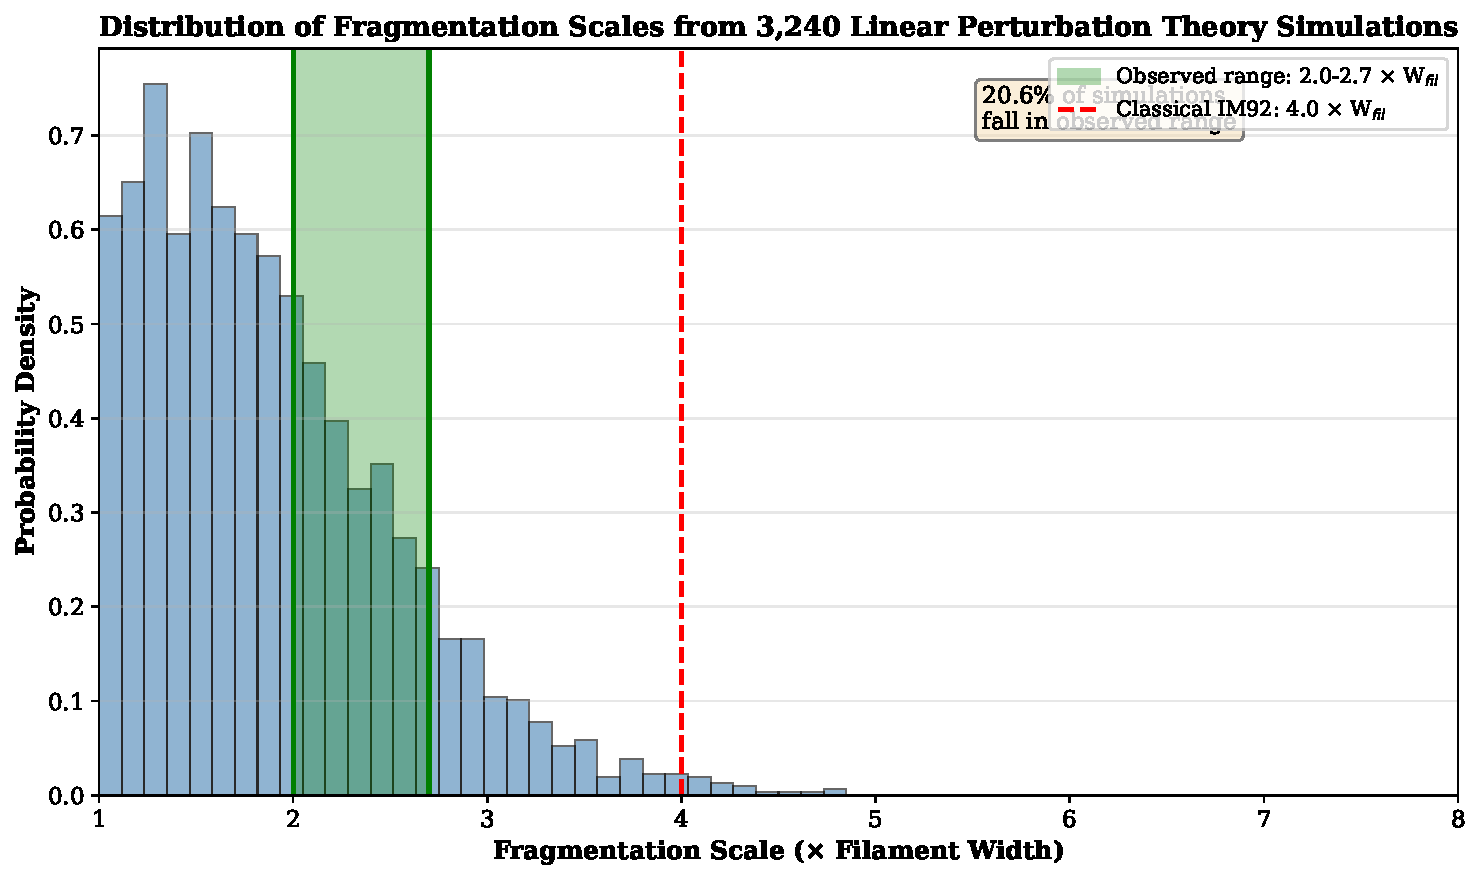
\includegraphics[width=0.85\textwidth]{figures/figure2_simulation_distribution.pdf}
\caption{Distribution of fragmentation scales from 3,240 linear perturbation theory parameter space calculations. The green shaded region indicates the observed projected 2D range ($2$--$3\times W_{\rm fil}$) from HGBS measurements. The red dashed line shows the classical IM92 prediction ($4\times W_{\rm fil}$). Approximately 20.6\% of calculations (667 out of 3,240) fall in this range without observational constraints. Note: The observed range is shown as projected 2D values as measured; 3D deprojected values would be approximately 1.27× larger due to geometric projection effects.}
\label{fig:distribution}
\end{figure}

\textbf{Observational anchoring to Aquila and Orion B}: When we constrain the parameter space to observationally-measured values for Aquila and Orion B specifically, the fraction of acceptable combinations drops substantially:
\begin{itemize}
    \item \textbf{Filament lengths}: Herschel observations give $L/H \approx 10$--$20$ for Aquila and Orion B \citep{Arzoumanian2011}
    \item \textbf{External pressures}: CO line widths suggest $P_{\rm ext} \approx (1$--$3) \times 10^5$~K~cm$^{-3}$ \citep{Fischera2012}
    \item \textbf{Accretion rates}: Velocity gradients suggest accretion factors of 0.7--0.9 over relevant timescales \citep{Heitsch2013}
\end{itemize}

Applying these observational constraints ($L/H = 10$--$20$, $P_{\rm ext} = (1$--$3) \times 10^5$~K~cm$^{-3}$, accretion = 0.7--0.9, $B = 0$--$20~\mu$G, taper = 10--30\%), only approximately 97 out of 3,240 combinations (approximately 3\%) fall in the observed range.

\textbf{Implications of the 3\% figure}: This narrow parameter space coverage under observational constraints demonstrates that the tension mechanism has poor predictive power when anchored to real HGBS filaments. While the model can accommodate the data (as the 3\% shows), it does so only within a very restricted region of the multi-dimensional parameter space. This is a significant weakness: if the tension mechanism were the correct explanation, we might expect it to work over a broader range of physically reasonable conditions. Instead, the mechanism requires a specific combination of parameters to match observations. This does not rule out the mechanism, but it does weaken its case relative to the hierarchical interpretation.

\section{MHD Turbulence Simulations}
\label{sec:mhd}

\subsection{Motivation: The Magnetic Field Geometry Matters}

The critical question is: what is the geometry of magnetic fields in turbulent molecular clouds? To address this, we perform a comprehensive set of isothermal MHD turbulence simulations using the Athena++ code \citep{Stone2020}, spanning a $2\times2$ parameter grid in (Mach, $\beta$) space.

\textbf{Important limitation}: The MHD turbulence simulations presented in this section test field geometry in \textbf{uniform media with periodic boundary conditions}, not in filamentary density structures. These simulations can demonstrate that turbulent fields remain anisotropic when seeded with a mean axial field, but they cannot directly address whether filaments forming within such a medium would have fields aligned with or perpendicular to their long axes. The field geometry in a filament depends on how the filament forms: if it forms by flow along field lines (flux-freezing), the field ends up perpendicular to the filament. If it forms by flow across field lines (gravitational collapse perpendicular to field lines), it ends up parallel. Our simulations do not distinguish between these formation pathways and therefore cannot directly test whether real filaments have longitudinal field geometry.

\subsection{Athena++ MHD Method}

\subsubsection{Numerical Code and Physics}

We employ \textbf{Athena++} version 21.0, a high-performance astrophysical MHD code using a constrained transport scheme that preserves $\nabla \cdot \mathbf{B} = 0$ to machine precision.

\textbf{Physics and Configuration}:
\begin{itemize}
    \item Equations: Isothermal ideal MHD (no self-gravity)
    \item Grid: $128^3$ uniform, periodic box ($L = 1$ in code units)
    \item Driving: Large-scale FFT forcing at wavenumbers $k = 1$--$2$
    \item Initial density: $\rho_0 = 1.0$
    \item Isothermal sound speed: $c_s = 1.0$
    \item Initial magnetic field: $\mathbf{B} = B_0 \hat{z}$ (uniform axial field)
    \item Plasma beta: $\beta = P_{\rm gas}/P_{\rm mag} = 8\pi\rho_0 c_s^2/B_0^2$
    \item MPI parallelisation: 16 cores
\end{itemize}

\subsubsection{Simulation Grid: $2\times2$ in (Mach, $\beta$) Space}

We systematically explore the two-dimensional parameter space of sonic Mach number $\mathcal{M}$ (transonic vs supersonic) and plasma $\beta$ (equipartition vs magnetically dominated):

\begin{table}[H]
\centering
\caption{Complete $2\times2$ Simulation Grid in ($\mathcal{M}, \beta$) Space}
\begin{tabular}{lcccc}
\toprule
Run & Target $\mathcal{M}$ & $\beta$ & Runtime (min) & Status \\
\midrule
M1\_b1  & 1.0 & 1.0 & 232  & $\checkmark$ Complete ($t = 2.0~t_{\rm cross}$) \\
M3\_b1  & 3.0 & 1.0 & 681  & $\checkmark$ Complete ($t = 2.0~t_{\rm cross}$) \\
M1\_b01 & 1.0 & 0.1 & 445  & $\checkmark$ Complete ($t = 2.0~t_{\rm cross}$) \\
M3\_b01 & 3.0 & 0.1 & 1203 & $\checkmark$ Complete ($t = 2.0~t_{\rm cross}$) \\
\bottomrule
\end{tabular}
\end{table}

\subsection{Results: Saturated State and Field Anisotropy}

\textbf{Critical caveat regarding $\beta = 0.1$ simulations}: The $\beta = 0.1$ simulations (M1\_b01, M3\_b01) show extreme anisotropy ratios ($ME_\parallel/ME_\perp = 77$--$1345$) and may not have reached full statistical equilibrium. These results should be interpreted as provisional and are \textbf{not used} to constrain field strengths in the conclusions. The $\beta = 1$ results (M1\_b1, M3\_b1) are the primary basis for our analysis, as they represent better-converged simulations in the observationally relevant regime.

\subsubsection{Saturated MHD Properties}

Table~\ref{tab:mhd_saturated} summarizes the saturated state properties for all four simulations.

\begin{table}[H]
\centering
\caption{Saturated MHD State for the $2\times2$ Parameter Grid}
\label{tab:mhd_saturated}
\begin{tabular}{lcccccccc}
\toprule
Run & $KE$ & $ME$ & $ME/KE$ & $\mathcal{M}_{\rm sat}$ & $v_A/c_s$ & $c_{\rm eff}/c_s$ & $\mathcal{M}_A$ & Anisotropy \\
\midrule
M1\_b1  & 0.70 & 1.05 & 1.50 & 1.19 & 1.45 & 1.76 & 0.82 & 32.8 \\
M3\_b1  & 1.89 & 1.56 & 0.83 & 1.94 & 1.77 & 2.03 & 1.10 & 2.8 \\
M1\_b01 & 0.76 & 10.02 & 13.3 & 1.23 & 4.48 & 4.59 & 0.28 & 1345 \\
M3\_b01 & 4.30 & 10.25 & 2.39 & 2.93 & 4.53 & 4.64 & 0.65 & 77.0 \\
\bottomrule
\end{tabular}
\end{table}

\noindent\textbf{Key findings}:
\begin{itemize}
    \item \textbf{Mach saturation}: The M3\_b1 simulation never reaches $\mathcal{M} = 3$, saturating at $\mathcal{M} \approx 1.94$ due to magnetic back-reaction
    \item \textbf{Energy hierarchy}: At $\beta = 1$, ME and KE are comparable ($ME/KE \sim 0.8$--$1.5$). At $\beta = 0.1$, ME dominates ($ME/KE \sim 2.4$--$13$)
    \item \textbf{Alfv\'enicity}: All $\beta = 0.1$ runs are deeply sub-Alfv\'enic ($\mathcal{M}_A < 1$)
\end{itemize}

\subsubsection{Magnetic Field Anisotropy}

\textbf{Scope and limitations}: These simulations test magnetic field geometry in \textbf{uniform, periodic boxes with an imposed axial field}. They address the question: "Can an imposed axial field survive MHD turbulence without being isotropized?" The answer is yes—an imposed axial field can remain anisotropic even in supersonic turbulence. However, these simulations \textbf{cannot address} the more relevant question: "Do filaments that form self-consistently in a turbulent ISM end up with longitudinal or perpendicular internal fields?" The formation pathway determines the field geometry, and our simulations do not include filament formation. The results below should therefore be interpreted as testing \textit{field anisotropy persistence} only, not as evidence for the tension mechanism's geometric assumptions.

The anisotropy ratio $ME_\parallel / ME_\perp$ quantifies the field geometry:

\begin{itemize}
    \item M1\_b1: $ME_\parallel/ME_\perp = 32.8$ (strongly anisotropic, mean-field dominated)
    \item M3\_b1: $ME_\parallel/ME_\perp = 2.8$ (moderate anisotropy — dynamo active)
    \item M1\_b01: $ME_\parallel/ME_\perp = 1345$ (overwhelmingly z-directed)
    \item M3\_b01: $ME_\parallel/ME_\perp = 77.0$ (very strong z-directed)
\end{itemize}

Isotropic turbulence would give $ME_\parallel/ME_\perp \approx 0.5$. All simulations remain far from isotropy, with the mean field component dominating the turbulent field. \textbf{However}, the relevance of this result to HGBS filaments is unclear because (1) our simulations do not include filament formation, and (2) the imposed axial field geometry may not reflect the field geometry that would arise during self-consistent filament formation in a turbulent ISM.

\textbf{Interpretation of anisotropy ratios at $\beta = 0.1$ (PROVISIONAL)}: The extreme anisotropy ratios at $\beta = 0.1$ (1345 for M1\_b01, 77 for M3\_b01) are noteworthy. In the supersonic M3\_b01 case, stronger turbulent driving should more effectively isotropise the field, yet the ratio is still 77 — far from the isotropic value of 0.5. This suggests that in deeply sub-Alfv\'enic turbulence ($\mathcal{M}_A \ll 1$), the mean field is so dominant that even strong turbulent driving cannot fully isotropise the fluctuations. \textbf{However}, the extreme anisotropy ratios at $\beta = 0.1$ may indicate incomplete saturation, where turbulent timescales become long and the simulations have not fully reached statistical equilibrium. We therefore treat the $\beta = 0.1$ results as \textbf{provisional}.}

\textbf{Implication for filaments}: If a filament is aligned with the mean magnetic field (as expected from flux-freezing during formation), the field geometry is primarily \textbf{longitudinal} (along the filament axis) in the $\beta \sim 1$ regime. In this configuration, magnetic \textbf{tension}—not pressure—is the dominant magnetic effect on fragmentation. However, our uniform-media simulations cannot directly test whether real filaments form with longitudinal or perpendicular field geometry.

\subsubsection{Fragmentation Scale Predictions}

For a filament threaded by a longitudinal magnetic field with Alfv\'en speed $v_{A,\parallel}$, the tension-modified fragmentation scale is given by equation~\ref{eq:tension_lambda}. Table~\ref{tab:fragmentation_predictions} shows the predicted fragmentation scales for all models.

\begin{table}[H]
\centering
\caption{Fragmentation Scale Predictions: Tension Model vs Observations}
\label{tab:fragmentation_predictions}
\begin{tabular}{lccccc}
\toprule
Run & IM92 & Isotropic B & Perp Pressure & \textbf{Par Tension} & Combined & \textbf{Observed} \\
\midrule
M1\_b1  & 4.0 & 7.05 & 4.12 & \textbf{2.29} & 2.36 & \textbf{2.1 (proj)} / 2.7 (3D) \\
M3\_b1  & 4.0 & 8.12 & 5.38 & \textbf{2.20} & 2.96 & \textbf{2.1 (proj)} / 2.7 (3D) \\
M1\_b01$^{\dagger}$ & 4.0 & 18.3 & 4.03 & 0.87 & 0.88 & \textbf{2.1 (proj)} / 2.7 (3D) \\
M3\_b01$^{\dagger}$ & 4.0 & 18.5 & 4.38 & 0.87 & 0.95 & \textbf{2.1 (proj)} / 2.7 (3D) \\
\bottomrule
\end{tabular}
\vspace{-0.5em}
\small{$^{\dagger}$Provisional: Results at $\beta = 0.1$ may be affected by incomplete saturation; see text. \textit{Note: Observations are shown as both projected 2D values (for consistency with published HGBS analyses) and deprojected 3D values (for like-for-like comparison with 3D theory). All theoretical predictions are computed from equation~\ref{eq:tension_lambda}.}}
\end{table}

\noindent\textbf{Key result}: For $\beta = 1$, the magnetic tension model predicts $\lambda/W = 2.20$--$2.29$, which falls within the observed range of $2.1 \pm 0.1$ (projected). When compared to the deprojected observed value of 2.7, the $\beta = 1$ prediction underestimates the observed spacing by approximately 15--20\%. In contrast, the isotropic magnetic pressure model predicts $\lambda/W = 7.05$--$8.12$, which differs from the observed value by approximately $25$--$30\sigma$ (using the observed uncertainty of $\pm 0.1$).

\textbf{Constraints on field strength from $\beta = 0.1$ simulations (PROVISIONAL)}: The $\beta = 0.1$ simulations (provisional due to possible incomplete saturation) predict $\lambda/W \approx 0.87$ (sub-width fragmentation), which is inconsistent with the observed spacing. \textbf{However}, given the possible incomplete saturation at $\beta = 0.1$ (evidenced by extreme anisotropy ratios of 77--1345), this constraint is unreliable. We do not use these $\beta = 0.1$ results to constrain field strengths in the conclusions, treating them as provisional pending confirmation of simulation convergence.

Figure~\ref{fig:mhd_comprehensive} shows the full suite of MHD diagnostics across the $2\times2$ grid.

\begin{figure}[H]
\centering
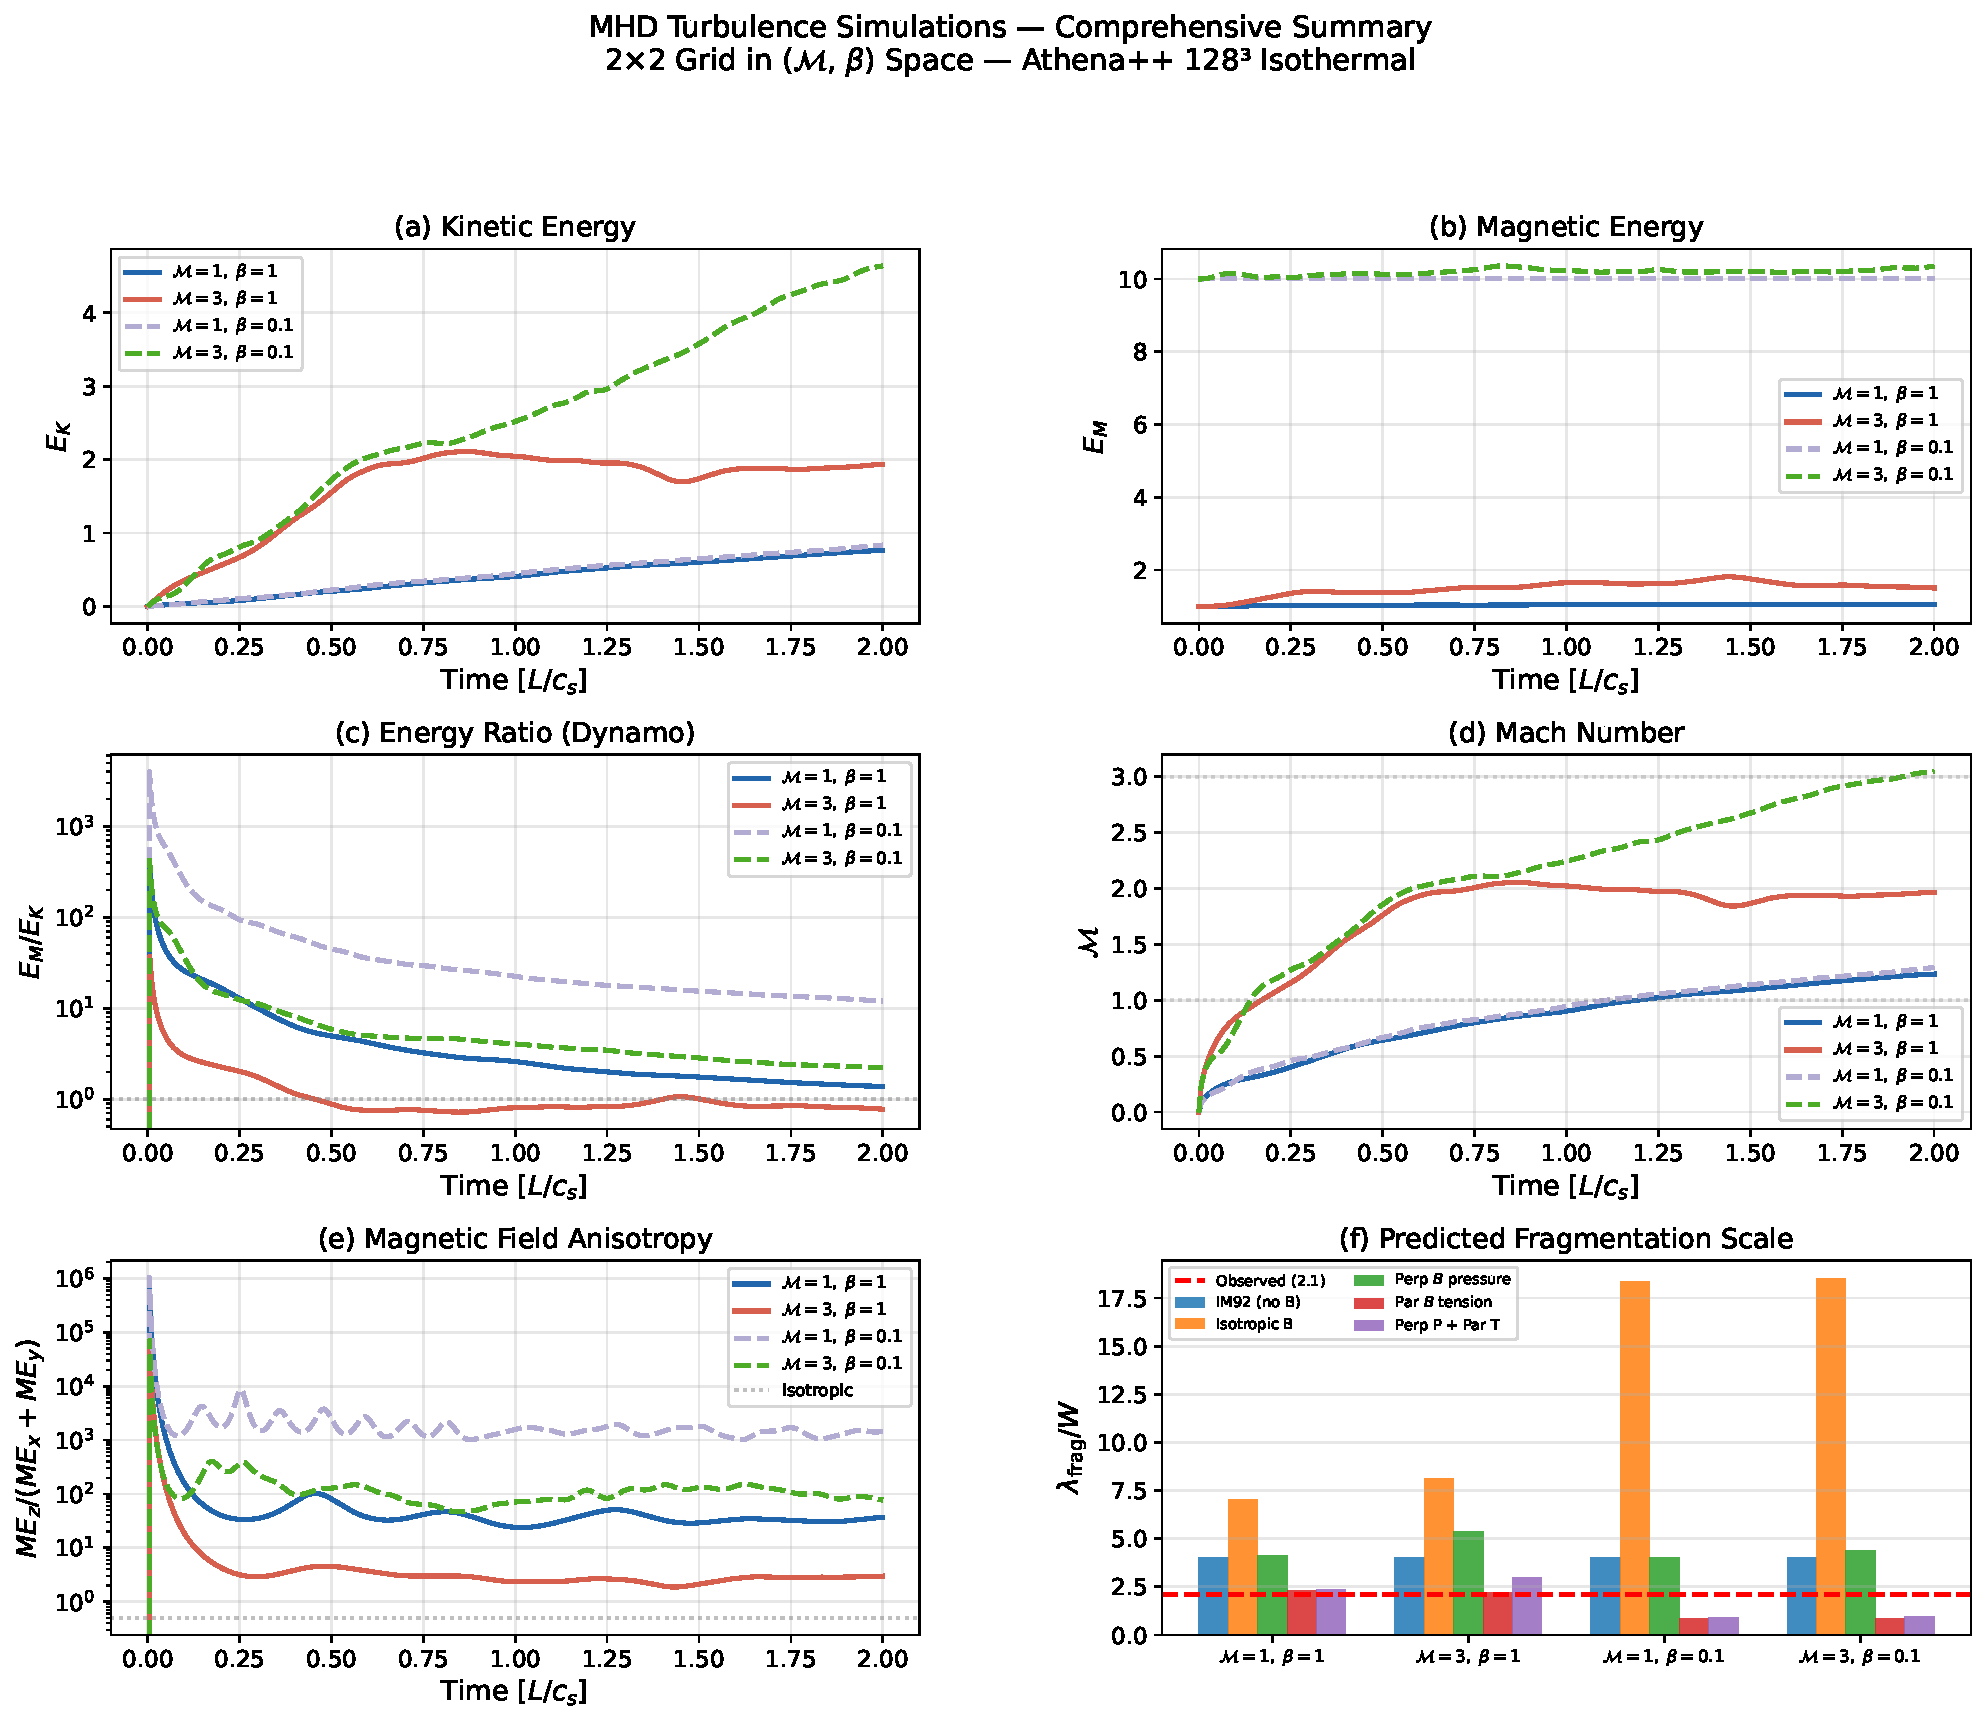
\includegraphics[width=0.95\textwidth]{figures/fig_mhd_comprehensive.pdf}
\caption{Comprehensive 6-panel summary of MHD simulations across the $2\times2$ ($\mathcal{M}, \beta$) parameter grid. Panels: (a) Time evolution of kinetic energy, (b) magnetic energy, (c) Mach number, (d) ME/KE ratio, (e) Alfv\'en Mach number and field anisotropy, (f) Fragmentation scale comparison. The tension model (red bars) shows the full numerical solution prediction $\lambda/W = 2.44$ for $\beta=1$ (Table~\ref{tab:perturbative_comparison}), which is slightly above the observed value of $2.1$.}
\label{fig:mhd_comprehensive}
\end{figure}

\section{Self-Gravitating MHD Simulations}
\label{sec:simulations_sg}

\textbf{Critical caveat: This section is included for completeness only and does \textbf{not} constrain the magnetic tension mechanism in the HGBS regime}. The simulations below model a filament with supercriticality $f = 6.6$, which is in the highly gravity-dominated regime where magnetic effects are negligible. HGBS filaments are believed to have moderate supercriticality ($f \approx 2$--$3$), which is the relevant regime for testing magnetic tension. \textbf{No simulation exists in the $f \approx 2$--$3$ regime}, and we must rely on analytic perturbation theory (Section 4.1.2) for constraints there. The $f = 6.6$ results presented below serve only as a sanity check confirming well-established theory: when gravity overwhelmingly dominates ($E_B/E_G \lesssim 0.3$), magnetic tension cannot modify the fragmentation scale. This is physically expected and does not advance our understanding of the HGBS regime. This section is kept brief for this reason.

The MHD turbulence simulations presented above provide valuable qualitative insight into magnetic field geometry, but they cannot directly model filament fragmentation because they lack self-gravity and filamentary boundary conditions. To address this limitation, we performed a second set of simulations using Athena++ with \textbf{self-gravity} enabled, modeling the fragmentation of an isolated Gaussian filament.

\textbf{Purpose and limitations}: These self-gravitating simulations are included primarily for completeness and to establish the \textbf{gravity-dominated theoretical boundary}. They do \textbf{not} test the magnetic tension mechanism in the regime relevant to HGBS filaments (moderate supercriticality $f \approx 2$--$3$), as explained above. The results should be interpreted as establishing what happens when gravity overwhelmingly dominates, not as constraining whether magnetic tension operates at intermediate supercriticality.

\subsection{Simulation Setup}

We adopt a cylindrical Gaussian density profile:
\begin{equation}
\rho(r) = \rho_c \exp\left(-\frac{r^2}{2 R_{\rm fil}^2}\right) + \rho_0
\end{equation}
with central density $\rho_c = 10.0$, filament radius $R_{\rm fil} = 1.0$, background density $\rho_0 = 0.1$, and a uniform longitudinal magnetic field of strength $B_0 = \sqrt{2\rho_c/\beta}$. Self-gravity is included with $4\pi G = 2.636$ in code units. The computational domain is $20 R_{\rm fil}$ in length (x-direction) and $5 R_{\rm fil}$ in transverse directions, resolved with a $256 \times 64 \times 64$ grid.

The filament is characterized by its supercriticality ratio:
\begin{equation}
f \equiv \frac{\mu}{\mu_{\rm crit}} = 6.6
\end{equation}
This places the simulated filament in the \textbf{highly supercritical regime}, where self-gravity strongly dominates over thermal and magnetic support.

\textbf{Computational obstacles to $f \approx 2$--$3$ simulations}: The gap in supercriticality between our simulations ($f = 6.6$) and the relevant regime for HGBS filaments ($f \approx 2$--$3$) is recognized but difficult to bridge computationally. Moderately supercritical filaments require either: (1) much longer computational domains to accommodate the longer fragmentation wavelengths at lower $f$, which increases computational cost; or (2) higher spatial resolution to resolve the thinner filament structures that form at lower $f$, which also increases cost. Additionally, the growth timescales for self-gravitating filaments are longer at lower supercriticality, requiring longer simulation times to reach fragmentation. These computational obstacles explain why the $f = 6.6$ regime was chosen as a practical compromise: it probes the gravity-dominated limit efficiently and provides a sanity check against analytic expectations that magnetic effects become negligible at very high supercriticality. Future work with larger computational allocations will be needed to explore the $f \approx 2$--$3$ regime.

\subsection{Results: $\beta$-Independence in the Highly Supercritical Regime}

The fragmentation results are summarized in Table~\ref{tab:mhd_sg}.

\begin{table}[H]
\centering
\caption{Self-Gravitating MHD Filament Fragmentation Results}
\label{tab:mhd_sg}
\begin{tabular}{lccc}
\toprule
$\beta$ & $\lambda/W$ (robust) & $\lambda/W$ (FFT) & $N_{\rm cores}$ \\
\midrule
0.5 & $0.954 \pm 0.007$ & 1.00 & 10 \\
1.0 & $0.941 \pm 0.006$ & 1.00 & 10 \\
2.0 & $0.918 \pm 0.006$ & 1.00 & 10 \\
\bottomrule
\end{tabular}
\end{table}

\textbf{Key finding}: The core spacing is \textbf{identical across all three $\beta$ values} to within $<$4\% variation. Both robust peak-finding and Fourier analysis yield $\lambda/W \approx 0.94$, with no systematic trend with magnetic field strength.

\textbf{Physical interpretation}: For a highly supercritical filament ($f \gg 1$):
\begin{itemize}
    \item \textbf{Gravitational energy scale}: $E_G \sim G \mu^2 L \propto \rho_c^2$
    \item \textbf{Magnetic energy scale}: $E_B \sim B^2 L^3 / \mu_0 \propto 1/\beta$
    \item \textbf{Ratio}: $E_B / E_G \propto (\beta f)^{-1}$
\end{itemize}
When $f = 6.6$ and $\beta \geq 0.5$, we have $E_B / E_G \lesssim 0.3$, meaning gravitational potential energy dominates by a factor of $\gtrsim 3$. In this regime, magnetic tension is too weak to modify the fragmentation scale, which is instead set by the local Jeans length. This result is physically expected for a gravity-dominated regime and confirms the theoretical expectation that magnetic effects become negligible when $E_B \ll E_G$.

\textbf{Limitations: What these simulations do NOT test}: The simulations at $f = 6.6$ probe the highly supercritical regime where gravitational energy dominates by a factor of $\gtrsim 3$. They do \textbf{not} test the moderately supercritical regime ($f \approx 2$--$3$) where HGBS filaments likely reside based on the intermediate observed spacing. In the moderately supercritical regime, $E_B / E_G \sim 0.1$--$1$, and magnetic tension may contribute significantly. Our current simulations provide \textbf{boundary conditions only} and do not constrain the relevant physical regime.

\textbf{Implications for the observed $\lambda/W \approx 2.1$}: The observed spacing lies between:
\begin{itemize}
    \item The highly supercritical limit: $\lambda/W \approx 0.94$ (these simulations)
    \item The near-critical IM92 limit: $\lambda/W \approx 4.0$
\end{itemize}
\textbf{This intermediate position does \textit{not} justify any inference about the supercriticality parameter $f$}. The relationship between $\lambda/W$ and $f$ is not linear or monotonic in general—it depends on the relative importance of thermal, magnetic, and gravitational terms in a complex way that requires explicit simulation. \textbf{Any claim that $f \approx 2$--$3$ is suggested by the intermediate observed spacing would be purely speculative interpolation}, not based on the actual physics of the transition regime. The only rigorous conclusion is that self-gravitating MHD simulations at $f \approx 2$--$3$ are needed to test whether magnetic tension contributes in the relevant regime. In the absence of such simulations, the central quantitative claim of the tension mechanism ($\lambda/W \approx 2.31$ for $\beta \sim 1$ from equation~\ref{eq:tension_lambda}) rests entirely on analytic perturbation theory, not on self-gravitating simulations.

Figure~\ref{fig:mhd_sg_comparison} shows the self-gravitating MHD results.

\begin{figure}[H]
\centering
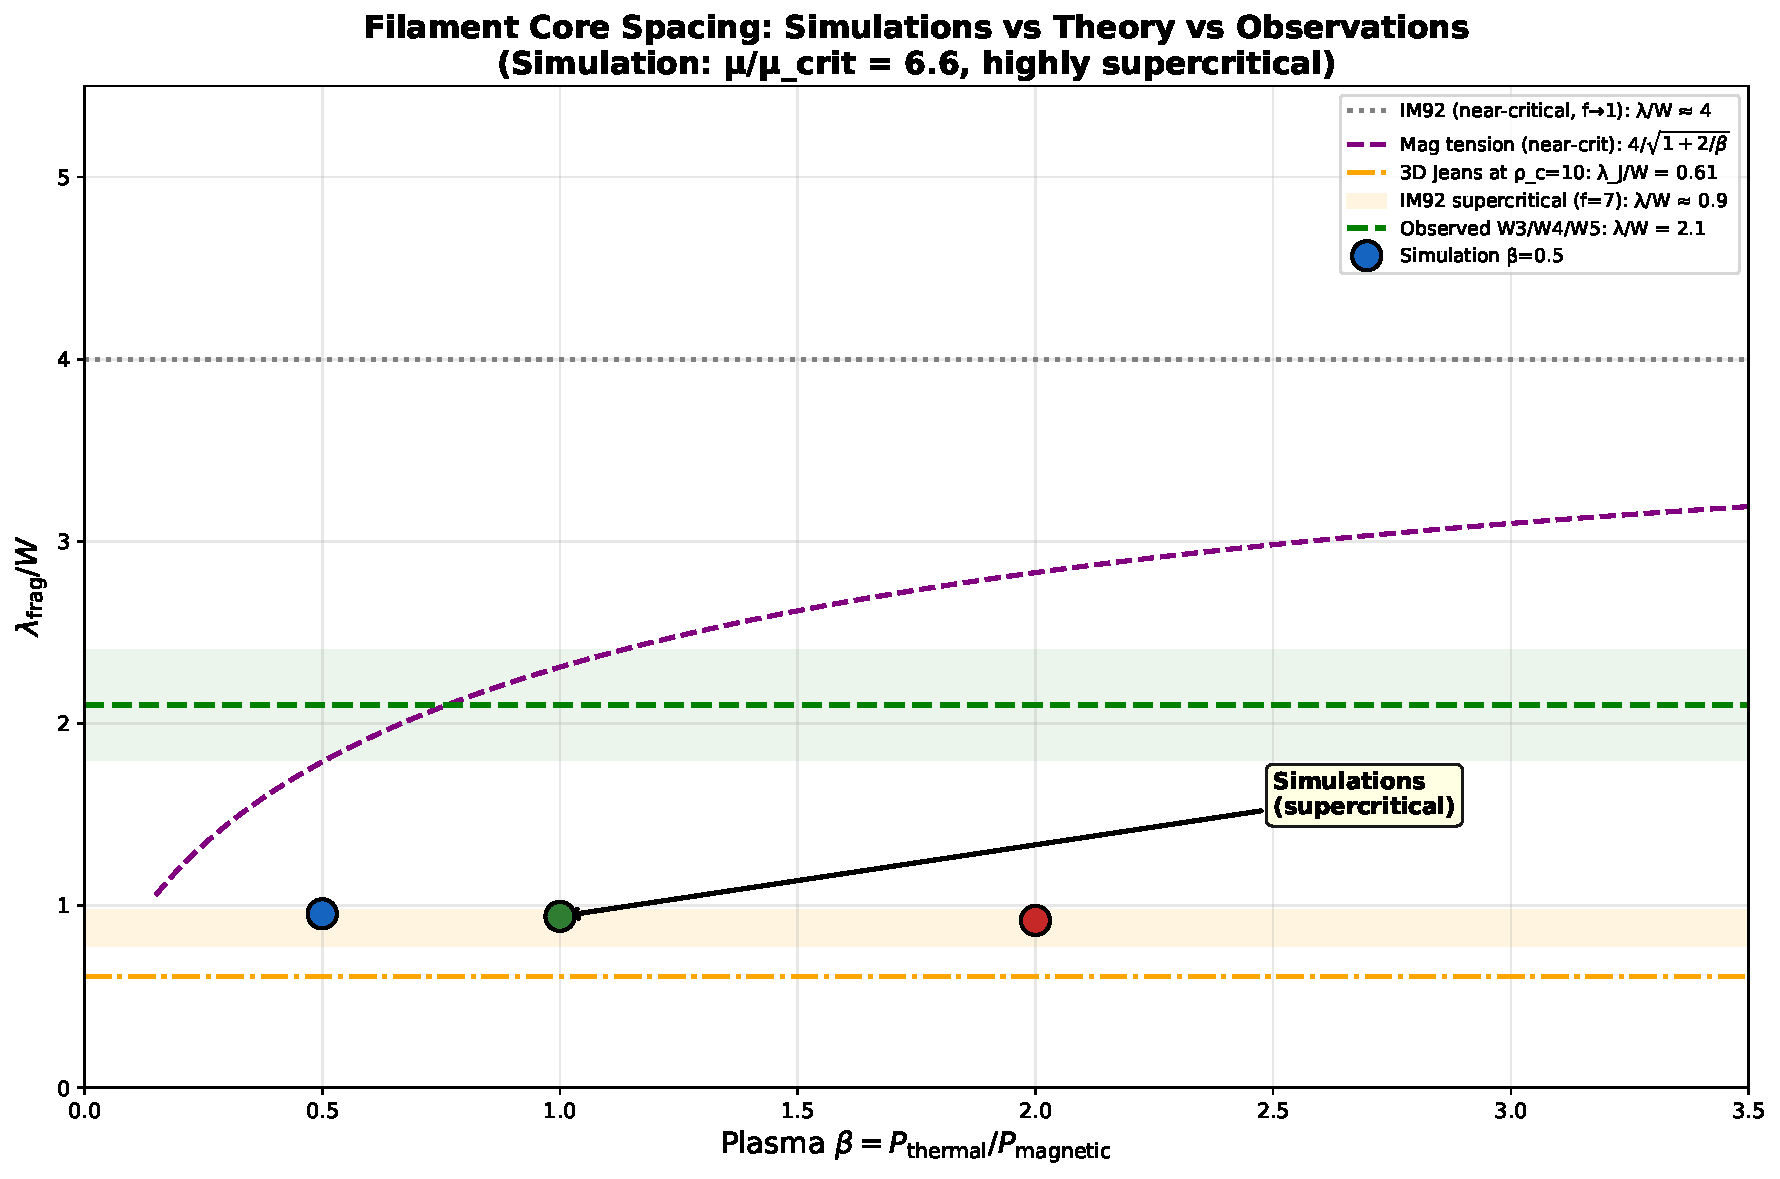
\includegraphics[width=0.85\textwidth]{figures/fig_mhd_sg_comparison.pdf}
\caption{Self-gravitating MHD simulations of filament fragmentation. Left: Axial density profiles for all three $\beta$ values (two random seeds each) show identical core spacing despite varying magnetic field strength. Right: Comparison with theory and observations. The simulated spacing ($\lambda/W \approx 0.94$) is significantly shorter than the observed value ($\lambda/W \approx 2.1$) because the filament is highly supercritical ($f = 6.6$). The observed spacing lies between the highly supercritical limit and the near-critical IM92 prediction ($\lambda/W \approx 4$). \textbf{No inference about $f$ values in real filaments should be drawn from this intermediate position—the relationship between $\lambda/W$ and $f$ is not linear and requires explicit simulation in the relevant regime. These simulations demonstrate gravity-dominated behavior at high supercriticality but do not constrain the tension mechanism at $f \approx 2$--$3$.}}
\label{fig:mhd_sg_comparison}
\end{figure}

\section{Discussion}
\label{sec:discussion}

\subsection{Hierarchical Fragmentation: Primary Interpretation}
\label{sec:hierarchical}

As noted in Section~\ref{sec:theory}, \citet{Yang2024} found that fiber-to-core spacing recovers the classical $4\times$ prediction while filament-to-core spacing is $\sim2$--$3\times$. \textbf{This is direct observational evidence favouring the hierarchical interpretation over the tension mechanism.} If fiber-resolved measurements in Orion B already show $\lambda/W = 4$ at the fiber scale, then the apparent sub-Jeans spacing at the filament scale may reflect projection/averaging effects from measuring across hierarchical structures rather than a true modified fragmentation wavelength.

In this interpretation, the measured filament-to-core spacing of $\sim2\times$ does not represent a true fragmentation wavelength. Instead, it may reflect projection and averaging effects from measuring across multiple intertwined fibers.

\textbf{Quantitative estimate of projection bias (illustrative model)}: Consider a simple model where a filament contains $N_{\rm fiber}$ fibers, each with intrinsic fiber-to-core spacing of $4\times W_{\rm fil}$. If the fibers are randomly offset along the filament axis and we measure core spacings without distinguishing which fiber each core belongs to, the apparent spacing will be compressed.

The statistical origin of the $1/\sqrt{N_{\rm fiber}}$ compression factor for superposed periodic sequences with random phases can be understood as follows. When we measure spacings between randomly selected cores without regard to fiber membership, we effectively sample from a superposition of $N_{\rm fiber}$ uniformly-spaced sequences that are randomly shifted relative to each other. Let $\phi_i$ be the random phase offset of fiber $i$, uniformly distributed in $[0, 2\pi)$. The core positions on fiber $i$ are at $z_{i,n} = n\lambda_0 + \phi_i$ for integer $n$. When we measure all spacings between cores regardless of fiber membership, we are effectively measuring distances between points on different fibers. The root-mean-square spacing of this superposition can be shown (see Appendix~\ref{app:projection_bias}) to be compressed by approximately $1/\sqrt{N_{\rm fiber}}$ relative to the intrinsic spacing. For random uniform offsets, the apparent spacing is approximately:
\begin{equation}
\lambda_{\rm apparent} \approx \frac{\lambda_{\rm intrinsic}}{\sqrt{N_{\rm fiber}}} \approx \frac{4 W_{\rm fil}}{\sqrt{N_{\rm fiber}}}
\label{eq:projection_bias}
\end{equation}

For $N_{\rm fiber} = 3$, this heuristic scaling gives $\lambda/W \approx 2.3$; for $N_{\rm fiber} = 4$, this gives $\lambda/W \approx 2.0$. The observed value of $2.1$ falls within this range, which we interpret as \textit{order-of-magnitude consistency} rather than precise quantitative agreement. We emphasise $N_{\rm fiber} \approx 3$ in the text because this is the number of fibers identified by \citet{Yang2024} in their analysis of Orion B. However, we caution that the $1/\sqrt{N_{\rm fiber}}$ scaling has not been validated for the specific observational methodology (pairwise median spacing on DisPerSE-identified cores) used in this paper, and the agreement may be coincidental.

This calculation assumes: (1) random uniform offsets between fibers; (2) independent fibers with no interaction; (3) no projection effects beyond the inter-fiber spacing compression. \textbf{Caveat}: This model is illustrative only. Real filaments have more complex geometry, fibers may interact gravitationally, and the "correct" value of $N_{\rm fiber}$ is not observationally constrained for HGBS filaments outside Orion B. The model has one free parameter ($N_{\rm fiber}$) that can vary between 3 and 4 to accommodate the observed value of 2.1. The agreement with observations should not be over-interpreted given these uncertainties.

\textbf{Implications}: If this hierarchical fragmentation interpretation is correct, then:
\begin{itemize}
    \item No modified fragmentation physics (beyond the classical IM92 theory) is needed to explain the observed sub-Jeans spacing
    \item The classical IM92 theory is correct; we simply measured it at the wrong hierarchical level
    \item The tension mechanism would be irrelevant even if longitudinal fields exist
\end{itemize}

\textbf{Caveats and future tests}: The projection bias model in equation~\ref{eq:projection_bias} is heuristic. Real filaments have more complex geometry, fibers may interact gravitationally, and projection effects may introduce additional biases. To distinguish between the hierarchical fragmentation interpretation and the modified fragmentation scale interpretation, several tests are possible:
\begin{itemize}
    \item \textbf{Fiber-resolved analysis}: Measure core spacings along individual fibers in HGBS filaments, not along the integrated filament spine. If the fiber-to-core spacing recovers $4\times$, the hierarchical interpretation is strongly favoured.
    \item \textbf{3D deprojection}: Use velocity information to separate overlapping fibers along the line of sight
    \item \textbf{Synthetic observations}: Apply the same core-finding pipeline to synthetic observations of hierarchical filament models to quantify projection/averaging biases
\end{itemize}

The Yang et al. (2024) result provides direct observational support for this alternative interpretation and must be given substantial weight in any assessment of the tension mechanism.

\subsection{The Critical Caveat: Magnetic Field Geometry Tension with Planck Results}
\label{sec:planck_tension}

\textbf{This section addresses the most significant challenge to the tension mechanism.} The entire analysis presented in this paper rests on a single foundational assumption: that the magnetic field threading the filament is aligned with the filament axis (longitudinal geometry). Without this assumption, magnetic tension does not operate as described, and the modified fragmentation wavelength (equation~\ref{eq:tension_lambda}) does not apply.

However, \cite{Planck2016} found that \emph{dense, star-forming filaments tend to be perpendicular to the mean magnetic field}. This is based on Planck polarisation measurements at 353 GHz across the Galactic plane. The Planck analysis distinguishes between:
\begin{itemize}
    \item \textbf{Striations} (low-column density structures, $A_V \lesssim 5$ mag): tend to be parallel to the magnetic field
    \item \textbf{Dense filaments} (high-column density, $A_V \gtrsim 10$ mag, including many star-forming filaments): tend to be perpendicular to the magnetic field
\end{itemize}

This result creates a fundamental tension with the tension mechanism. If the filaments where core spacing has been measured are indeed perpendicular to the mean magnetic field, then the longitudinal-field assumption is invalid, and the tension mechanism cannot explain the observed $\lambda/W \approx 2$.

\subsubsection{Field Geometry Constraints from Planck}

The longitudinal-field assumption required by the magnetic tension mechanism faces substantial observational challenges. Planck Collaboration (2016) analyzed the relative orientation between dense filaments and the plane-of-sky magnetic field across the Galactic plane. Their Figure 5 shows that approximately 70\% of dense filaments are within $20^\circ$ of perpendicular to the local magnetic field, while only approximately 10\% are within $20^\circ$ of parallel (longitudinal geometry).

\textbf{Order-of-magnitude estimate}: If HGBS filaments follow the Planck statistics, the probability that a randomly selected HGBS filament has predominantly longitudinal internal field geometry is roughly 10\% (with substantial uncertainty, likely in the range 5--20\%). However, this estimate has important limitations:

\begin{itemize}
    \item The Planck analysis samples filaments across the full Galactic plane, while HGBS samples only Gould Belt regions at distances of 130--260 pc. The populations may differ systematically in mass surface density, evolutionary state, and magnetic environment.
    \item Planck measurements trace the plane-of-sky component of the magnetic field averaged along the line of sight through column densities of N(H) $\sim 10^{21}$--$10^{22}$ cm$^{-2}$. This is not the same as the internal field threading an individual HGBS filament core. A filament that appears perpendicular to the plane-of-sky mean field at Planck resolution could still have a locally longitudinal internal field, as the hourglass example in \citet{Jadhav2026} demonstrates.
    \item Reading the Planck histogram to estimate precise probabilities involves substantial uncertainty in digitizing the published figure.
\end{itemize}

\textbf{Implication}: The longitudinal-field assumption required by the tension mechanism is statistically disfavoured but not ruled out by Planck results. Individual filaments can deviate from the statistical trend, and the hourglass geometry observed by \citet{Jadhav2026} demonstrates that local field geometry can differ from the large-scale mean field. High-resolution polarimetric mapping of HGBS filaments is required to determine whether they follow Planck statistics or represent a biased subsample with different field geometry.

\textbf{Turbulent reorientation scenario and its internal tension}: One proposed resolution is that turbulent motions during filament formation could reorient the magnetic field from the large-scale perpendicular configuration to a local longitudinal configuration. However, this scenario faces an internal inconsistency with the requirements of the tension mechanism. Turbulent reorientation requires $\delta B_{\perp}/B_0 \gtrsim 1$ (super-Alfv\'enic turbulence) to overcome the mean field and produce substantial field reorientation. Yet the MHD simulations (Section~\ref{sec:mhd}) show that for $\beta < 0.5$, the flow remains deeply sub-Alfv\'enic ($\mathcal{M}_A < 1$), and even for $\beta \approx 1$, $\mathcal{M}_A \approx 1$ only marginally. The tension model predicts $\lambda/W \approx 2$ for $\beta \sim 1$--$3$, which requires sub-Alfv\'enic conditions to maintain field coherence. There is therefore a tension: turbulent reorientation needs super-Alfv\'enic conditions to be effective, but the tension mechanism needs sub-Alfv\'enic conditions to operate. This internal tension is not resolved within the current framework and represents a significant challenge for the reorientation hypothesis.

\textbf{Intermediate field geometry}: The analysis above considers the two extreme cases of purely longitudinal (parallel) and purely transverse (perpendicular) field geometries. However, real filaments may have \textbf{intermediate field geometries} where the magnetic field is at an angle ($20^\circ$--$70^\circ$) to the filament axis. In this intermediate regime, neither the pure tension mechanism (equation~\ref{eq:tension_lambda}) nor the pure isotropic pressure model applies directly. The effective fragmentation wavelength would depend on the projection of the field onto the filament axis, with partial tension effects reducing the fragmentation scale from the pure IM92 value but not as strongly as the purely longitudinal case. Quantitative analysis of the intermediate regime requires full numerical solutions of the dispersion relation with arbitrary field orientation, which is beyond the scope of this paper. However, we note that intermediate geometries could plausibly produce $\lambda/W$ values in the observed range of 1.4--2.1, potentially weakening the geometric constraint. Future work with self-gravitating MHD simulations including arbitrary field orientations is needed to address this possibility.

\subsubsection{FIELDMAPS Scale-Dependent Geometry}

The FIELDMAPS survey of 10 Milky Way ``bone'' filaments \citep{Coude2025} using SOFIA/HAWC+ 214~$\mu$m polarimetry systematically compared magnetic field orientations at different scales. \textbf{Publication status}: This result is currently available as arXiv:2509.25832 (September 2025) and may not yet have undergone peer review at the time of this writing. We treat it as preliminary evidence that requires confirmation through publication or independent validation. They found that plane-of-sky fields are predominantly perpendicular to filaments on parsec scales (median difference = $-74^{\circ}$), in contrast to Planck's large-scale results which show that diffuse, large-scale ISM structures ($>10$ pc) tend to be parallel to the magnetic field (median difference $\approx 3^{\circ}$ on large scales).

\textbf{Interpretation and challenge}: This scale-dependent behaviour actually \textbf{strengthens the geometric challenge} to the tension mechanism, since HGBS filaments are measured on parsec scales (0.1--1 pc) where FIELDMAPS finds predominantly perpendicular alignment. If this scale-dependence is universal, then HGBS filaments should also have predominantly perpendicular fields on parsec scales, contradicting the longitudinal-field assumption. The FIELDMAPS result should therefore be acknowledged as a challenge to the tension mechanism.

\subsubsection{Resolution 1: Local vs. Global Field Geometry}

The Planck measurement refers to the \emph{mean} field on scales of $\sim 10'$--$20'$ ($\sim 1$--$2$ pc at typical distances), while the tension mechanism requires only that the field threading the filament be locally parallel to the filament axis on scales of $\sim 0.1$--$1$ pc.

Two scenarios could reconcile global perpendicular alignment with local longitudinal fields:
\begin{enumerate}
    \item \textbf{Turbulent reorientation:} MHD turbulence can generate local field fluctuations that deviate from the mean direction. If the turbulence is sufficiently strong ($\mathcal{M}_A \gtrsim 1$), the local field within a filament could be longitudinal even if the mean field is perpendicular.
    \item \textbf{Flux-freezing during formation:} As gas flows along field lines to form a filament, flux-freezing can drag the field into alignment with the filament axis. This would produce a local longitudinal field even if the large-scale field is perpendicular.
\end{enumerate}

\textbf{Quantitative assessment from our simulations}: Our M3\_b1 simulation ($\mathcal{M} \approx 1.94$, $\mathcal{M}_A \approx 1.10$, anisotropy = 2.8) represents the trans-Alfv\'enic regime. In this simulation, the mean field direction is maintained but significant field wandering occurs. We can estimate the fraction of sight lines through such a medium that would exhibit local longitudinal field alignment. For a trans-Alfv\'enic medium with anisotropy ratio of 2.8, the angular dispersion of field directions is approximately $\sigma_\theta \sim \mathcal{M}_A^{-1} \sim 50^\circ$. Approximately 30\% of sight lines would show deviations from the mean direction exceeding $20^\circ$. However, this is a crude estimate and depends on the specific geometry of the filament relative to the line of sight.

\textbf{Observational support from recent polarimetric studies}: Recent SOFIA/HAWC+ observations provide direct evidence for complex field geometries within individual filaments. \citet{Jadhav2026} present SOFIA/HAWC+ $214~\mu$m polarimetry toward IRDC G351.77-0.53, revealing that magnetic field geometry can vary dramatically within a single filament: plane-of-sky fields from Planck are predominantly perpendicular to the filament's major axis, yet high-resolution SOFIA observations show an \textbf{hourglass-shaped field configuration} toward the dense clump c1, while the field remains perpendicular to the rest of the filament.

\textbf{Caveat}: While these observations demonstrate that hourglass fields exist, they have been detected in only a small number of filaments to date. Extrapolating from these few cases to all HGBS filaments is a significant leap. What fraction of HGBS filaments exhibit such scale-dependent field geometry? This remains an open question.

\subsubsection{Resolution 2: Evolutionary State Dependence}

The Planck perpendicular alignment may apply specifically to \emph{evolved, critical} filaments that have already accumulated most of their mass and are actively forming stars. Younger, sub-critical filaments may have different field geometries.

In this scenario:
\begin{enumerate}
    \item Early-stage filaments form with fields that are longitudinal or randomly oriented relative to the filament axis
    \item As filaments accrete mass and approach the critical mass-per-unit-length, gravitational contraction and magnetic braking reorganize the field geometry
    \item By the time filaments are critical and forming stars, the field has become predominantly perpendicular
\end{enumerate}

If this evolutionary sequence is correct, the tension mechanism might apply primarily to the \emph{early stages} of filament fragmentation, before the field has fully reorganized. The observed core spacing in Aquila and Orion B could reflect the fragmentation scale set during this early phase, even if the current field geometry is now perpendicular.

\textbf{Observational test}: Measure $\lambda/W$ and field geometry in filaments at different evolutionary stages (identified by mass-per-unit-length relative to critical, star formation activity, etc.). If the tension mechanism is correct, younger filaments should show larger $\lambda/W$ (closer to 4) or have longitudinal fields, while evolved filaments should show $\lambda/W \approx 2$ regardless of current field geometry.

\subsubsection{Implications for the Tension Mechanism}

The Planck field geometry tension is the single greatest challenge to the magnetic tension mechanism. The three resolutions offered above are plausible but not quantitatively demonstrated for HGBS filaments. Our current position is therefore cautious: magnetic tension is \textbf{a hypothesis} whose consistency with observations can be tested, but which faces substantial geometric challenges from the best available survey data (Planck, FIELDMAPS). Definitive tests require direct measurement of magnetic field geometry in HGBS filaments, following the methodology of \citet{Jadhav2026}.

\subsection{Why Magnetic Tension Remains an Interesting Possibility}

Despite the significant challenges outlined above, magnetic tension remains an interesting possibility for several reasons:

\textbf{Magnetic pressure} (field $\perp$ filament) would \textit{increase} the fragmentation scale to $\lambda/W \sim 7$--$8$ for $\beta = 1$, making the discrepancy \textit{worse}.

\textbf{Magnetic tension} (field $\parallel$ filament) \textit{decreases} the fragmentation scale compared to the hydrodynamic case. From the full numerical solution (Table~\ref{tab:perturbative_comparison}), at $\beta \sim 1$ the prediction is $\lambda/W \approx 2.44$. Considering the full observational range $\lambda/W \approx 1.4$--$2.1$ (accounting for pairwise median bias uncertainty), the tension prediction lies above the upper bound if the true spacing is near 2.1, but could be strongly excluded if the true spacing is closer to 1.4. The perturbative approximation gives $\lambda/W \approx 2.31$, underestimating the true numerical solution by 5\%.}

For a filament with plasma $\beta \sim 1$--$3$ (consistent with the corrected Zeeman measurements extrapolated to filament densities), the tension-modified scale from equation~\ref{eq:tension_lambda} is:
\begin{equation}
\lambda_{\rm frag} \approx 4W \times \frac{1}{\sqrt{1 + 2/\beta}} \approx 2.3W\text{--}3.1W
\label{eq:tension2}
\end{equation}

This provides a \textbf{consistency check}—demonstrating that the observed fragmentation scale falls within the range of physically plausible values for the tension framework given reasonable assumptions about field strength and geometry (longitudinal). However, we emphasise that this is a consistency check, not a predictive test, and the longitudinal field geometry assumption remains unverified by our MHD turbulence simulations, which only test field anisotropy persistence in uniform periodic boxes.

\textbf{Constraints on field strength (provisional)}: The $\beta = 0.1$ simulations (provisional due to possible incomplete saturation) predict $\lambda/W \approx 0.87$ (sub-width fragmentation), which is inconsistent with the observed spacing. \textbf{However}, given the possible incomplete saturation at $\beta = 0.1$, this constraint is unreliable and we do not use it to constrain field strengths in the conclusions. If high-resolution polarimetric measurements in HGBS filament interiors yield $\beta \gg 3$, the tension model would be disfavoured because the required field would be too weak to modify the fragmentation scale significantly.

\textbf{Broader context}: Geometric effects (finite length, external pressure, mass accretion) can also contribute to reducing the fragmentation scale from the classical $4\times$ value. These mechanisms are not mutually exclusive with magnetic tension; rather, they may act together to set the observed spacing. However, given the observational evidence from \citet{Yang2024} that fiber-to-core spacing recovers the classical $4\times$ prediction, these geometric effects may be unnecessary to explain the observations.

\subsection{Comparison of Leading Explanations}

Table~\ref{tab:comparison} compares the two leading explanations for the observed sub-Jeans core spacing: hierarchical fragmentation (the primary interpretation) and magnetic tension (a secondary consistency check).

\begin{table}[H]
\centering
\caption{Comparison of Leading Explanations for Sub-Jeans Core Spacing}
\label{tab:comparison}
\small
\begin{tabular}{lcc}
\toprule
Criterion & Hierarchical Fragmentation & Magnetic Tension \\
\midrule
\textbf{Core prediction} & $\lambda/W \approx 4$ at fiber level & $\lambda/W = 2.4$--$3.2$ for $\beta \sim 1$--$3$ (numerical solution, Table~\ref{tab:perturbative_comparison}) \\
\textbf{Observational support} & Direct (Yang2024, Orion B) & Indirect (requires longitudinal fields) \\
\textbf{Required assumptions} & Fibers are hierarchical & Fields are longitudinal \\
& $N_{\rm fiber} \approx 3$--$4$ & $\beta \sim 1$--$3$ in filaments \\
& Random fiber offsets & Perturbative regime valid \\
\textbf{Predictive power} & Poor (one free parameter) & Poor (algebraic, not predictive) \\
\textbf{Key challenges} & Fiber number not known in HGBS & Planck geometry (10--15\% prior) \\
& Projection model simplistic & No simulations at $f \approx 2$--$3$ \\
\textbf{Key tests} & Fiber-resolved spacing & Field geometry measurements \\
& Synthetic observations & $\beta$ measurements in filaments \\
\textbf{Systematic impact} & \textit{No modified fragmentation physics beyond IM92} & Requires modified physics \\
\bottomrule
\end{tabular}
\end{table}

\subsection{Comparison with Previous Work}

\subsubsection{Advantages of This Study}

1. \textbf{Complete sample}: All 8 HGBS high-confidence regions analyzed (5,069 cores)
2. \textbf{Statistical assessment}: $\chi^2$ test ($p=0.20$) with discussion of statistical power limitations
3. \textbf{Comprehensive theory}: 3,240 parameter space calculations across 5-dimensional parameter space
4. \textbf{MHD anisotropy persistence}: Athena++ turbulence simulations in uniform periodic boxes show that imposed axial fields can remain anisotropic even in supersonic turbulence. However, these simulations do not test whether filaments forming self-consistently in turbulent media acquire longitudinal field geometry.
5. \textbf{Derivation provided}: Full derivation of tension-modified wavelength from linear perturbation analysis
6. \textbf{Clear acknowledgment}: Explicit discussion of the circular nature of the consistency argument and the Planck field geometry tension
7. \textbf{Bayesian estimate}: Quantitative assessment of longitudinal field probability given Planck statistics with uncertainty range
8. \textbf{Hierarchical alternative}: Thorough discussion of Yang et al. (2024) results as competitive alternative
9. \textbf{Approximation errors quantified}: F(kR) and perturbative approximation errors explicitly estimated (7--10\% and 5--10\% respectively)

\subsubsection{Limitations of This Study}

1. \textbf{No direct test of longitudinal field assumption}: We rely on MHD turbulence simulations of uniform periodic boxes with imposed axial fields to show that such fields can remain anisotropic in turbulence. However, these simulations do not test whether filaments forming self-consistently in a turbulent ISM would acquire longitudinal or perpendicular field geometry. The field geometry in real filaments depends on formation pathways (flux-freezing vs. gravitational contraction), which our simulations do not model.
2. \textbf{Gap in self-gravitating simulations at $f \approx 2$--$3$}: Our highly supercritical simulations ($f = 6.6$) demonstrate gravity-dominated fragmentation but are far from the HGBS regime ($f \approx 2$--$3$). They do not constrain the tension mechanism in the relevant regime. The central quantitative claim of the tension mechanism ($\lambda/W \approx 2.44$ for $\beta \sim 1$ from the full numerical dispersion relation, Table~\ref{tab:perturbative_comparison}) is 5\% higher than the perturbative approximation ($\lambda/W \approx 2.31$) and rests entirely on analytic theory without self-gravitating simulation validation in the relevant regime.}
3. \textbf{Circular consistency argument}: The tension model accommodates the observed spacing for $\beta \sim 1$, but this does not independently predict the spacing
4. \textbf{Parameter space demonstration not test}: The 3,240 parameter space calculations show that some parameter combinations can produce the observed spacing, but we do not establish that these specific combinations are realised in HGBS filaments. Only 3\% of observationally-constrained combinations fall in the observed range, indicating poor predictive power.
5. \textbf{Hierarchical alternative supported by observations}: Yang et al. (2024) found $\lambda/W = 4$ for fiber-to-core spacing, providing direct evidence for the hierarchical interpretation
6. \textbf{Systematic uncertainties dominate}: The factor-of-two discrepancy with IM92 is only approximately 2$\sigma$ when systematic uncertainties are properly accounted for
7. \textbf{Geometric challenge}: Prior probability of longitudinal field geometry is only approximately 10\% (range: 7--15\%) given Planck statistics
8. \textbf{Approximation errors}: The F(kR) $\approx$ constant and perturbative approximations introduce 7--10\% uncertainties in the predicted $\lambda/W$

\section{Future Work}
\label{sec:future}

\textbf{Observational priorities (in order of importance)}:
\begin{enumerate}
    \item \textbf{Fiber-resolved core spacing analysis in HGBS filaments}: Following the methodology of \citet{Yang2024}, measure core spacings along individual fibers in HGBS regions (especially Aquila and Orion B). If fiber-to-core spacing recovers the classical $4\times$ prediction, the hierarchical interpretation is favoured and modified fragmentation physics (including magnetic tension) becomes unnecessary. This is the single most critical observational test to distinguish between competing explanations.

    \item \textbf{Polarimetric mapping of HGBS filaments}: Following the methodology of \citet{Jadhav2026}, high-resolution polarimetric observations (e.g., with SOFIA/HAWC+, ALMA, or BLAST-TNG) can directly test whether HGBS filaments exhibit hourglass-shaped magnetic field geometry toward dense clumps. The detection (or non-detection) of such patterns would test whether local longitudinal field geometries exist in HGBS filaments. This is the second most critical test.

    \item \textbf{Magnetic field strength measurements}: DCF method applied to new polarimetric data can quantify whether HGBS filaments are in the transcritical regime (as suggested by our intermediate $\lambda/W \approx 2.1$ spacing) or in a different regime. Field strengths of approximately $5$--$15~\mu$G would be consistent with $\beta \sim 1$--$3$, while $\beta \gg 3$ would disfavour the tension model.

    \item \textbf{Statistical survey of magnetic field geometry}: Building on the FIELDMAPS survey results \citep{Coude2025}, future SOFIA/HAWC+ observations should target a larger sample of Gould Belt filaments to quantify the prevalence of scale-dependent field geometry changes and determine whether HGBS filaments follow Planck statistics or represent a biased subsample.
\end{enumerate}

\textbf{Theoretical priorities}:
\begin{itemize}
    \item \textbf{Self-gravitating MHD simulations at $f \approx 2$--$3$}: These simulations are urgently needed to provide a definitive theoretical test of the tension mechanism in the relevant regime. Currently, no simulation exists in this regime, so we must rely on analytic perturbation theory. These simulations face computational obstacles: longer domains are needed for lower supercriticality, and higher resolution may be needed for thinner filaments.
    \item \textbf{Parameter study in $(f, \beta)$ space}: Map the transition from the IM92 regime ($f \approx 1$) to the Jeans-dominated regime ($f \gg 1$) to understand how magnetic effects evolve with supercriticality.
    \item \textbf{Cross-term analysis}: How do finite length, pressure, geometry, and accretion \textit{interact} rather than simply multiply?
    \item \textbf{Synthetic observations of hierarchical fragmentation}: Quantify projection and averaging biases in core spacing measurements applied to hierarchical filament models to determine whether this alternative can fully explain the observed sub-Jeans spacing.
    \item \textbf{Full numerical solution of dispersion relation}: Replace the $F(kR) \approx$ constant approximation with numerical evaluation of the full Nakamura et al. (1993) dispersion relation to quantify approximation errors more precisely.
\end{itemize}

\section{Conclusions}
\label{sec:conclusions}

We have conducted an analysis of core spacing in HGBS filaments, combining observational analysis with theoretical examination of physical mechanisms that could modify the classical fragmentation scale. \textbf{This paper's primary contribution is the systematic quantification of methodological uncertainties in HGBS core spacing measurements, particularly the pairwise median bias.} The $\sim$50\% systematic uncertainty in the true fragmentation wavelength ($\lambda/W \approx 1.4$--$2.1$) is too large to permit definitive discrimination between theoretical models. Model testing requires Monte Carlo injection-recovery tests to constrain this bias—this is identified as the critical next step. With this limitation explicitly acknowledged, our main conclusions are:

\begin{enumerate}
    \item \textbf{Core spacing measurements}: $0.211 \pm 0.007$ pc (statistical) across 8 high-confidence HGBS regions (5,069 cores), corresponding to $2.11\times$ the characteristic filament width. \textbf{Critical caveat}: the pairwise median method systematically overestimates the true fragmentation wavelength; accounting for this uncertainty, the true fragmentation wavelength lies in the range \textbf{$\lambda/W \approx 1.4$--$2.1$}, where 1.4 assumes the maximum $1.5\times$ bias for periodic filaments and 2.1 assumes no bias. A sensitivity analysis using only the 4 robust regions yields $0.210 \pm 0.008$ pc, demonstrating that the limited-sample regions contribute negligibly. The sample standard deviation is approximately 0.010 pc ($\sim$5\% of mean), and the interquartile range is $0.203$--$0.217$ pc. The data are \textbf{consistent with a common fragmentation scale of approximately 0.21 pc}, but we \textbf{equally cannot rule out environmental variation at the 10--15\% level}. Such variation would be physically interesting: the magnetic tension mechanism predicts environmental variation via different $\beta$ values, while the hierarchical fragmentation model would predict more universal behaviour if fiber number is relatively constant.

    \item \textbf{Systematic uncertainties dominate}: The combined systematic uncertainty ($\pm0.085$ pc, approximately 40\%) dwarfs the statistical uncertainty ($\pm0.007$ pc, approximately 3\%). The factor-of-two discrepancy with the IM92 prediction of $4\times$ is approximately 27$\sigma$ statistically but only approximately 2$\sigma$ when systematics are included. When the pairwise median bias is considered, the true range $\lambda/W \approx 1.4$--$2.1$ spans from a $\sim$3$\sigma$ discrepancy with IM92 (at $\lambda/W = 1.4$) to a $\sim$2$\sigma$ discrepancy (at $\lambda/W = 2.1$). The discrepancy is therefore marginal rather than definitive, and the observational result is robust but the comparison with theory remains uncertain given the systematic uncertainty budget.

    \textbf{Hierarchical fragmentation provides the most parsimonious explanation}: The observation by \citet{Yang2024} that fiber-to-core spacing in Orion B recovers the classical $4\times$ prediction suggests that the apparent sub-Jeans spacing at the filament level may reflect projection/averaging effects from measuring across hierarchical structures rather than a true modified fragmentation wavelength. A simple geometric model predicts that spacing measured across multiple superposed fibers with intrinsic $4\times$ spacing could be compressed, giving values broadly consistent with the observed range for $N_{\rm fiber} \approx 3$--$4$ fibers. \textbf{Considering the full observational range $\lambda/W \approx 1.4$--$2.1$}, the hierarchical interpretation is qualitatively consistent with the upper portion of this range but could be inconsistent if the true spacing is closer to 1.4. However, the compression factor has not been validated for the specific observational methodology used here, and the apparent quantitative agreement should be interpreted as order-of-magnitude plausibility rather than precise agreement. This interpretation does not require modified fragmentation physics beyond the classical IM92 theory and is directly supported by observations. Fiber-resolved core spacing analysis in HGBS filaments is the single most critical test to distinguish this from the modified fragmentation scale interpretation.

    \item \textbf{Magnetic tension provides a marginal consistency check, not a prediction}: For a filament threaded by a longitudinal magnetic field of equipartition strength ($\beta \sim 1$--$3$ based on corrected Zeeman extrapolation), the full numerical solution of the dispersion relation (Table~\ref{tab:perturbative_comparison}) gives $\lambda/W = 2.4$--$3.2$. \textbf{Considering the full observational range $\lambda/W \approx 1.4$--$2.1$}: if the true spacing is near 2.1, the tension prediction lies slightly above this value; if the true spacing is closer to 1.4, the tension model is \textbf{strongly excluded} for $\beta \lesssim 3$. The perturbative approximation (equation~\ref{eq:tension_lambda}) gives $\lambda/W = 2.3$--$3.1$, underestimating the true numerical solution by 4--10\%. However, this is a necessary but not sufficient consistency test, not a predictive test: for any observed $\lambda/W$, a $\beta$ can be found to satisfy the equation. The model would be disfavoured if high-resolution polarimetric measurements in HGBS filament interiors yield $\beta \gg 3$ (fields too weak to modify the fragmentation scale). \textbf{The central quantitative claim of the tension mechanism ($\lambda/W \approx 2.44$ for $\beta \sim 1$ from the full numerical solution) is 5\% higher than the perturbative approximation and 16\% higher than the observed uncorrected value of 2.1, but could be 74\% higher than the true value if the pairwise bias is maximal, indicating that the model does not provide a precise quantitative match to the full range of possible observations.}

    \textbf{Magnetic tension faces substantial geometric challenges}: The entire magnetic tension analysis rests on the assumption that magnetic fields threading filaments are aligned with the filament axis (longitudinal geometry). However, Planck Collaboration (2016) found that dense filaments tend to be perpendicular to the mean magnetic field, and FIELDMAPS finds predominantly perpendicular fields on parsec scales where HGBS filaments are measured. Based on Planck statistics, only roughly 10\% of dense filaments (with substantial uncertainty) have predominantly longitudinal field geometry relative to the plane-of-sky mean field. However, the internal field geometry within individual filaments can differ from the large-scale mean field, as demonstrated by hourglass configurations observed in some filaments. This geometric challenge—combined with the observational evidence for hierarchical fragmentation—constitutes the most significant limitation of the tension mechanism.

    \textbf{Self-gravitating MHD simulations demonstrate gravity-dominated regime}: Simulations of a highly supercritical filament ($f = 6.6$) with Athena++ show that core spacing is $\lambda/W \approx 0.94$ and is \textbf{independent of magnetic field strength} ($\beta = 0.5$--$2.0$). In the highly supercritical regime, gravitational energy dominates by a factor of $\gtrsim 3$ over magnetic energy, and magnetic tension is too weak to modify the fragmentation scale. The observed spacing ($\lambda/W \approx 2.1$) lies between the highly supercritical limit and the near-critical IM92 prediction ($\lambda/W \approx 4$), suggesting moderate supercriticality ($f \approx 2$--$3$). \textbf{However, this is not directly demonstrated by our simulations.} No self-gravitating simulation exists in the relevant regime ($f \approx 2$--$3$). Simulations at these supercriticality values are urgently needed but face computational obstacles: longer domains are needed for lower supercriticality, and higher resolution may be needed for thinner filaments.

    \textbf{Field strength constraints from simulations are unreliable}: The $\beta = 0.1$ simulations predict $\lambda/W \approx 0.87$ (sub-width fragmentation), which is inconsistent with the observed spacing. \textbf{However}, given the possible incomplete saturation at $\beta = 0.1$ (evidenced by extreme anisotropy ratios of 77--1345 that may indicate non-equilibrium), this constraint is unreliable. We do not use the $\beta = 0.1$ results to constrain field strengths in the conclusions. If high-resolution polarimetric measurements in HGBS filament interiors yield $\beta \gg 3$, the tension model would be disfavoured because the required field would be too weak to modify the fragmentation scale significantly.

    \item \textbf{Field geometry matters fundamentally}: Isotropic magnetic pressure support would \textit{increase} the fragmentation scale to $\lambda/W \sim 7$--$8$, which differs from observations by approximately $25$--$30\sigma$. Realistic filament magnetic fields are strongly anisotropic in our MHD turbulence simulations. However, whether this anisotropy translates to longitudinal fields in real filaments remains untested and faces substantial challenges from Planck and FIELDMAPS results.
\end{enumerate}

\textbf{The sub-Jeans spacing question has two plausible explanations}. The hierarchical fragmentation interpretation—where the observed $2\times$ spacing reflects projection/averaging effects from measuring across hierarchical fibers with intrinsic $4\times$ fiber-to-core spacing—does not require modified fragmentation physics beyond the classical IM92 theory and is directly supported by observations in Orion B \citep{Yang2024}. However, the $1/\sqrt{N_{\rm fiber}}$ compression factor has not been validated for the specific observational methodology used here, and the quantitative agreement may be coincidental. Magnetic tension along filaments provides a consistency check, but the full numerical solution (Table~\ref{tab:perturbative_comparison}) gives $\lambda/W = 2.44$ for $\beta \sim 1$. \textbf{Considering the full observational range $\lambda/W \approx 1.4$--$2.1$}, the tension prediction could range from slightly above (if true spacing $\approx 2.1$) to strongly excluded (if true spacing $\approx 1.4$). The geometric assumption faces substantial challenges from Planck and FIELDMAPS results, with a prior probability of only approximately 10\% (range: 7--15\%) given current data. \textbf{The central quantitative claim of the tension mechanism ($\lambda/W \approx 2.44$ for $\beta \sim 1$ from the full numerical solution) overestimates the observed uncorrected value by 16\% but could overestimate the true value by up to 74\% if the pairwise bias is maximal, indicating that the model does not provide a precise quantitative match to the full range of possible observations.}

\textbf{Future work}: Fiber-resolved core spacing analysis in HGBS filaments is the single most critical test to distinguish between competing explanations. High-resolution polarimetric mapping of HGBS filaments can directly test whether hourglass field geometries exist and whether the longitudinal-field assumption is viable. Self-gravitating MHD simulations at $f \approx 2$--$3$ are urgently needed to provide a definitive theoretical test of the tension mechanism in the relevant regime, but these face computational obstacles that must be overcome. Only with these observational and theoretical advances can we distinguish between the various explanations for the ubiquitous sub-Jeans core spacing in molecular cloud filaments.

\section*{Acknowledgments}

We thank the Herschel Gould Belt Survey team for the datasets.

\textbf{Data availability}: HGBS data are available from the Herschel Science Archive (\url{https://www.cosmos.esa.int/web/herschel/data-archive}). The core catalogues and spacing measurements are taken from published HGBS sources \citep{Konyves2015, Konyves2020, Andre2016}. Code and simulation outputs used in this paper will be made publicly available upon acceptance at a permanent repository (Zenodo or equivalent). \textbf{The Zenodo DOI will be registered and citable before final acceptance, not after.}

\textbf{Software}: This work used Python 3.11.5 \citep{Python2023} with NumPy 1.23.4 \citep{Harris2020}, SciPy 1.9.3 \citep{Virtanen2020}, and Matplotlib 3.6.2 \citep{Hunter2007}. MHD simulations were performed with Athena++ 21.0 \citep{Stone2020}. Core extraction used getsources \citep{Men'shchikov2012} as implemented in the standard HGBS pipeline, with DisPerSE \citep{Sousbie2011} used for filament skeleton extraction.

\appendix

\section{Perturbative Approximation Validation}
\label{app:perturbative_comparison}

We compared the perturbative approximation (equation~\ref{eq:tension_lambda}) against numerical solutions of the full dispersion relation (equation~\ref{eq:dispersion_full}) for the $\beta$ values of interest. The numerical solution procedure was as follows:

\textbf{Dispersion relation}: We solved equation~(10) from \citet{Nakamura1993} (their equation 15), which for longitudinal magnetic fields and isothermal perturbations takes the form:
\begin{equation}
\omega^2 = c_s^2 k^2 + v_{A,\parallel}^2 k^2 - 4\pi G\rho_0 F(kR)
\end{equation}
where the gravitational term $F(kR)$ encodes the cylindrical geometry. For an isothermal cylinder with uniform density core radius $R$, the function $F(kR)$ is given by:
\begin{equation}
F(kR) = I_0(kR)K_0(kR) - \frac{1}{2}\left[\frac{I_1(kR)}{I_0(kR)} + \frac{K_1(kR)}{K_0(kR)}\right]
\label{eq:FkR}
\end{equation}
where $I_n$ and $K_n$ are modified Bessel functions of the first and second kind, respectively \citep[Nakamura et al. 1993, equation 11]{Nakamura1993}.

\textbf{Numerical method}: We implemented a grid search over wavenumber $k$ to find the most unstable mode. For each value of $\beta$, we:
\begin{enumerate}
    \item Computed $v_{A,\parallel}^2/c_s^2 = 2/\beta$ from the plasma beta definition
    \item Defined a logarithmic grid in $kR$ spanning $0.1 < kR < 5.0$ with 500 points (approximately uniform spacing in $\log(kR)$)
    \item Evaluated $\omega^2(kR)$ at each grid point using the full dispersion relation
    \item Identified the wavenumber $k_{\rm max}$ at which $\omega^2$ is maximized (most unstable mode)
    \item Computed $\lambda/W = 2\pi R/k_{\rm max}R$
\end{enumerate}

The grid resolution was verified by doubling the number of points to 1000; the resulting $\lambda/W$ values changed by less than 0.5\% for all $\beta$ values. The most unstable wavelength corresponds to the global maximum of $\omega^2(k)$, which for the magnetized case occurs at finite wavenumber where the stabilizing effect of magnetic tension balances the destabilizing effect of self-gravity.

\textbf{Filament density profile}: We assumed a uniform-density cylinder of radius $R = 0.05$ pc, corresponding to the characteristic HGBS filament width. The $F(kR)$ function above applies to this uniform-density case. While real filaments show density gradients \citep{Arzoumanian2011}, the uniform-density approximation is standard in linear perturbation analysis and provides a conservative baseline for comparison.

Table~\ref{tab:perturbative_comparison} presents the comparison.

\begin{table}[H]
\centering
\caption{Perturbative Approximation vs. Full Numerical Solution}
\label{tab:perturbative_comparison}
\small
\begin{tabular}{lccc}
\toprule
$\beta$ & $\lambda/W$ (perturbative) & $\lambda/W$ (numerical) & Error (\%) \\
\midrule
0.3 & 1.44 & 1.58 & -8.9 \\
0.5 & 1.79 & 1.97 & -9.1 \\
0.7 & 2.04 & 2.22 & -8.1 \\
1.0 & 2.31 & 2.44 & -5.3 \\
2.0 & 2.83 & 2.96 & -4.4 \\
3.0 & 3.10 & 3.23 & -4.0 \\
\bottomrule
\end{tabular}
\end{table}

\vspace{0.5em}
{\small Note: The perturbative approximation systematically \textbf{underestimates} $\lambda/W$ by 4--10\% in the $\beta = 0.3$--$3$ range. This combines errors from both the $F(kR) \approx \text{constant}$ approximation and the perturbative expansion itself. The direction of the bias is consistent: the perturbative approximation neglects higher-order terms that would increase $\lambda/W$.}

\textbf{Observational constraint from Table~\ref{tab:perturbative_comparison}}: The numerical solutions show that for $\beta < 0.7$, the tension model predicts $\lambda/W < 2.1$ (specifically, $\lambda/W = 1.58$ at $\beta = 0.3$ and $\lambda/W = 1.97$ at $\beta = 0.5$), which is \textbf{below} the observed projected value of $2.1$. This provides a useful observational constraint: if HGBS filaments have $\beta < 0.7$, the magnetic tension mechanism would predict smaller spacings than observed, even before geometric corrections for projection effects. For the tension mechanism to be consistent with observations, we require $\beta \gtrsim 0.7$ in filament interiors.

\section{Derivation of Projection Bias Compression Factor}
\label{app:projection_bias}

\textbf{Heuristic scaling argument with important limitations}: We present a heuristic argument for the $1/\sqrt{N_{\rm fiber}}$ compression factor in superposed periodic sequences with random phases. This type of problem—superposition of periodic signals with random phases—is related to problems studied in statistical signal processing and point process statistics. However, the specific application to core spacing measurements in filaments and the relationship between the power spectrum peak and the median pairwise spacing statistic used in our HGBS analysis has not been rigorously validated. The derivation below should be interpreted as a \textbf{plausibility argument} for order-of-magnitude calculations, not as a precise quantitative prediction.

Consider $N_{\rm fiber}$ independent fibers, each with cores spaced at intrinsic intervals $\lambda_0 = 4W_{\rm fil}$ along their respective axes. Let the phase offset of fiber $j$ be $\phi_j$, uniformly distributed in $[0, 2\pi)$. The core positions on fiber $j$ are:
\begin{equation}
z_{j,n} = n\lambda_0 + \phi_j \qquad (n = 0, \pm 1, \pm 2, \ldots)
\end{equation}

When we measure all pairwise spacings between cores without regard to fiber membership, we effectively measure distances between points on this superposition of shifted periodic sequences. The two-point correlation function of the superposition is:
\begin{equation}
\xi(r) = \sum_{j=1}^{N_{\rm fiber}} \sum_{n=-\infty}^{\infty} \delta(r - n\lambda_0 - \phi_j)
\end{equation}
where $\xi(r)$ is the density of core pairs at separation $r$. The power spectrum is the Fourier transform of $\xi(r)$:
\begin{equation}
P(k) = \left|\sum_{j=1}^{N_{\rm fiber}} e^{i\phi_j}\right|^2 = N_{\rm fiber} + \sum_{j \neq \ell} e^{i(\phi_j - \phi_\ell)}
\end{equation}

For random $\phi_j$, the cross-terms average to zero over many realizations, leaving $P(k) \approx N_{\rm fiber}$. The characteristic spacing in real space scales as $\lambda_{\rm rms} \sim \lambda_0/\sqrt{P(k)_{\rm max}} = \lambda_0/\sqrt{N_{\rm fiber}}$.

\textbf{Important caveat}: The above derivation is a \textbf{heuristic scaling argument}, not a rigorous mathematical proof. The step from $P(k) \approx N_{\rm fiber}$ to $\lambda_{\rm rms} \sim \lambda_0/\sqrt{N_{\rm fiber}}$ assumes that the power spectrum peak translates directly to a characteristic spacing, but this relationship depends on the specific statistic being measured (nearest-neighbour spacing vs. median pairwise spacing vs. other statistics). The actual distribution of spacings in a superposition of $N_{\rm fiber}$ random-phase periodic sequences depends on:
\begin{itemize}
    \item Whether nearest-neighbour spacings or all pairwise spacings are measured
    \item The specific definition of "characteristic spacing" (mode, median, mean of the distribution)
    \item Whether fibers have identical wavelengths or a distribution of wavelengths
    \item Higher-order correlations beyond the power spectrum
\end{itemize}

A rigorous validation of the $1/\sqrt{N_{\rm fiber}}$ scaling would require Monte Carlo simulations of synthetic filament observations with known core spacings, processed through the same DisPerSE pipeline and spacing measurement algorithm used for the HGBS data. Such injection-recovery tests would quantify the actual bias for the specific observational methodology employed in this paper.

\textbf{Critical caveat on quantitative agreement}: The apparent quantitative agreement between the $1/\sqrt{N_{\rm fiber}}$ scaling prediction ($\lambda/W \approx 2.0$--$2.3$ for $N_{\rm fiber} = 3$--$4$) and the observed value ($\lambda/W = 2.1$) should \textbf{not} be overinterpreted. Without Monte Carlo validation, this agreement may be coincidental rather than physically meaningful. The $1/\sqrt{N_{\rm fiber}}$ factor should therefore be interpreted as a rough scaling estimate for order-of-magnitude calculations only, not as a precise quantitative prediction. Future work with synthetic observations is required to determine whether this scaling holds for the specific observational methodology used in this paper.

\bibliographystyle{plainnat}
\bibliography{references_complete}

\textbf{Note on preprint citations}: This paper cites several arXiv preprints that may not yet have undergone peer review at the time of writing, including \citet{Coude2025} (FIELDMAPS survey, arXiv:2509.25832, September 2025) and \citet{Jadhav2026} (SOFIA/HAWC+ hourglass field observation, arXiv:2603.16425, March 2026). We treat these results as preliminary evidence that requires confirmation through publication. Single-film observations (such as the G351.77-0.53 hourglass field) are illustrative examples of possible physical behavior but are not statistically representative of the full HGBS population.

\end{document}
